% =====================================================================
%  PLA DE TREBALL (PT) -- Concurs LE-403/729 (UPC)
%  Version 2 (16/11/2026), built on PT_skeleton.tex. American English, aligned with the
%  HAP (three research lines, HAP numbering of publications [J], [R], [C], [D]).
%  General context on the UPC, the EEBE and the subjects adapted from the PT of
%  J. Calafell and the Professor Agregat project, rewritten in English.
%  Personal data: ONLY name and surname (base 3.5).
%  Before submitting: uncomment \finaltrue to hide the marks.
%  Output file name: Monteiro_Carlos_PT.pdf
% =====================================================================
\documentclass[11pt]{article}
\usepackage{lector}
\usepackage{pgfgantt}
\usepackage{needspace}
\usetikzlibrary{arrows.meta,positioning}
\newcommand{\sectionbreak}{\clearpage}
% \NEW{...}: new or modified text, in red (plain text with \finaltrue)
\newcommand{\NEW}[1]{\iffinal #1\else{\color{red}#1}\fi}
%\finaltrue
\setupheader{PT}

\title{\textbf{Pla de Treball}\\[2pt]\large Work Plan}
\author{\Large \CandName}
\date{}

\begin{document}
\maketitle
\thispagestyle{plain}
\vspace{0.5cm}
\begin{center}\postdata\end{center}

\newpage
\tableofcontents

% =====================================================================
\section{Research plan}\label{sec:research}

My doctoral research focused on understanding the fundamental mechanisms governing turbulent flows under supercritical thermodynamic conditions, where strong variations in thermophysical properties influence flow dynamics and transport processes.
During my doctoral research at the Universitat Politècnica de Catalunya (UPC), I investigated these phenomena through direct numerical simulation (DNS), contributing to the detailed characterization of flow states and turbulence organization in wall-bounded supercritical flows under different thermophysical and buoyancy regimes [J2--J7]\footnote{My own publications are cited with the numbering of Section~3.4 of the \textit{Historial Acadèmic i Professional} (HAP): [J] articles in indexed journals; [R] submitted articles, proceedings and articles in preparation; [C] conference papers; and [D] datasets.}.
In parallel, I contributed to the development of RHEA-X, a GPU-native, high-fidelity flow solver designed to address the computational demands of multiphysics turbulence [J1].
My most recent research concerned the physical mechanisms underlying extreme thermal events, leading to the development of Lagrangian and information-theoretic (causality assessment) approaches during the 2026 Center for Turbulence Research (CTR) Summer Program at Stanford University [R2, R3].
These contributions establish the scientific and computational foundations for the research program proposed here.

\subsection{Research context and motivation}\label{sec:background}

Supercritical fluids offer significant opportunities to improve the efficiency, performance, and compactness of advanced energy and propulsion technologies \cite{Li2025,Guardone2024}.
In aerospace propulsion, liquid rocket engines frequently operate at pressures exceeding the critical pressures of their propellants.
As shown in Figure~\ref{fig:regen}a,b, these are first passed through regenerative cooling channels of thrust chambers and subsequently injected into high-pressure combustors~\cite{Nasuti2021,JofreUrzay2021}.
Computational design and additive manufacturing now produce increasingly complex cooling passages (Figures~\ref{fig:regen}a and~\ref{fig:duct}a)~\cite{LEAP71,Gradl2019}, whose design relies on accurate predictions of heat transfer at supercritical pressure.
High-pressure injection and film cooling further motivate the investigation of mixing and thermal protection under supercritical conditions.
In energy technologies, supercritical CO$_2$ (sCO$_2$) Brayton cycles offer high thermal efficiencies and substantially more compact turbomachinery than conventional steam-based systems, with applications in waste-heat recovery, energy storage, and nuclear and concentrated solar power generation \cite{Li2025,Guardone2024}.
These advantages are closely connected to the distinctive thermophysical properties of fluids operating at supercritical pressures, particularly near the pseudo-boiling region \cite{Banuti2015}.
In this region, pronounced variations in density, viscosity, thermal conductivity, and specific heat (Figure~\ref{fig:regen}c) can substantially modify turbulence, mixing, and heat transfer \cite{Li2025}.
Despite their efficiency advantages, supercritical fluids can exhibit heat-transfer deterioration (HTD) under certain conditions, causing severe localized wall-temperature rises that threaten component reliability (Figure~\ref{fig:regen}b) \cite{Pizzarelli2018,Nasuti2021,Li2025}.

\begin{figure}[t]
	\centering
	\def\FigH{5.15cm}%
	\begin{tabular}[b]{@{}c@{}}
		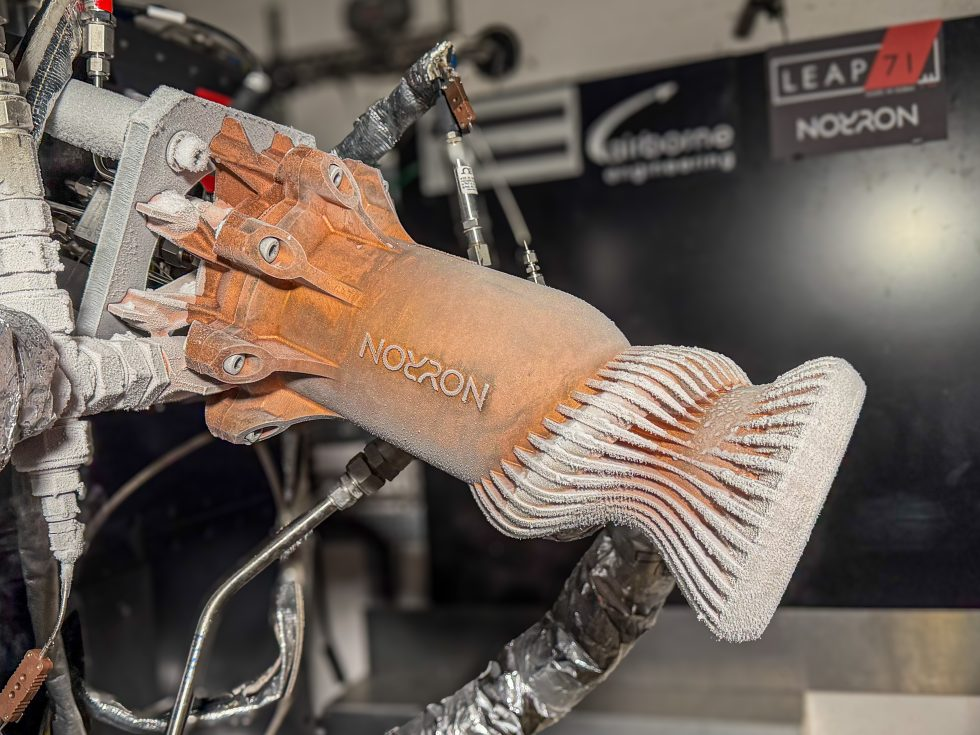
\includegraphics[height=\FigH, trim=120 0 40 0, clip]{images/leap71_engine.jpg}\\[-1pt]
		{\small (a)}
	\end{tabular}\hspace{2mm}%
	\begin{tabular}[b]{@{}c@{}}
		\resizebox{!}{\FigH}{\begin{tikzpicture}[font=\scriptsize\rmfamily, x=1cm, y=1cm,
				arr/.style={-{Stealth[length=1.5mm]}, line width=0.6pt}]
				% ---- cross-section A-A (top)
				\begin{scope}[shift={(0.45,2.75)}, scale=1.25]
					\fill[black!12] (0,0) rectangle (2.55,1.12);
					\foreach \x in {0.2,1.05,1.9} {
						\shade[top color=UPCAccent!35, bottom color=red!45] (\x,0.14) rectangle ++(0.45,0.84);
						\draw[black!60] (\x,0.14) rectangle ++(0.45,0.84);
						\draw[dashed, black!70] (\x,0.4) -- ++(0.45,0);
					}
					\foreach \x in {0.35,0.85,1.35,1.85,2.35} \draw[arr, red!70!black] (\x,-0.35) -- (\x,0.02);
					\node[red!70!black] at (1.27,-0.5) {$q_w$ (hot-gas side only)};
					\node[align=left, anchor=west] at (2.65,0.8) {liquid-like};
					\node[align=left, anchor=west] at (2.65,0.28) {gas-like};
					\draw[black!50] (2.35,0.75) -- (2.65,0.8); \draw[black!50] (2.35,0.25) -- (2.65,0.28);
					\node[anchor=south] at (1.27,1.12) {section A--A: cooling channels};
				\end{scope}
				% ---- thrust chamber and nozzle (upper half), wall with coolant passage
				\def\inner{(0,1.05) -- (1.4,1.05) .. controls (2.0,1.05) and (2.1,0.55) .. (2.5,0.55)
					.. controls (2.9,0.55) and (3.4,1.0) .. (4.3,1.45)}
				\def\outer{(0,1.40) -- (1.4,1.40) .. controls (2.0,1.40) and (2.1,0.90) .. (2.5,0.90)
					.. controls (2.9,0.90) and (3.4,1.35) .. (4.3,1.80)}
				\fill[orange!12] (0,0) -- \inner -- (4.3,0) -- cycle;
				\draw[line width=0.9pt, black!70] \inner;
				\draw[line width=0.9pt, black!70] \outer;
				\draw[black!40] (0,0) -- (4.3,0);
				\node[orange!70!black, align=center] at (0.85,0.55) {hot combustion\\ gas};
				\draw[arr, orange!80!black] (0.25,0.15) -- (1.45,0.15);
				\draw[arr, UPCAccent, line width=0.9pt] (4.15,1.62) .. controls (3.4,1.18) and (2.9,0.72) .. (2.5,0.72)
				.. controls (2.1,0.72) and (2.0,1.22) .. (1.4,1.22) -- (0.15,1.22);
				\node[UPCAccent, align=center, anchor=west] at (4.35,1.75) {coolant in\\ ($P>P_c$,\\ $T<T_{pb}$)};
				\node[UPCAccent, anchor=south] at (0.55,1.42) {to injector};
				\draw[arr, red!70!black] (2.5,0.15) -- (2.5,0.50);
				\node[red!70!black, align=center] at (2.5,-0.18) {throat: peak $q_w$};
				\draw[dashed, black!50] (1.8,1.6) -- (1.8,0.85) node[pos=0,above] {A};
		\end{tikzpicture}}\\[-1pt]
		{\small (b)}
	\end{tabular}\hspace{2mm}%
	\begin{tabular}[b]{@{}c@{}}
		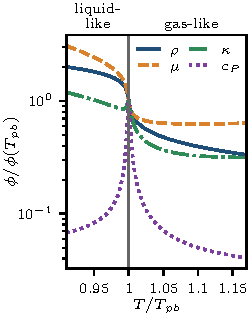
\includegraphics[height=\FigH]{images/co2_pseudoboiling_narrow.pdf}\\[-1pt]
		{\small (c)}
	\end{tabular}
	\caption{(a) Regeneratively cooled engine designed by LEAP~71; the frost on its surface is caused by the cryogenic propellant in the cooling passages (image:
		LEAP~71~\cite{LEAP71}). (b) Schematic of regenerative cooling at supercritical pressure through rectangular channels in the chamber wall; near the heated wall the coolant crosses $T_{pb}$ and becomes gas-like, which can trigger heat-transfer deterioration~\cite{Pizzarelli2018,Nasuti2021,Urbano2013}. 
		(c) Thermophysical properties of CO$_2$ at 8~MPa across the pseudo-boiling temperature $T_{pb}=307.8$~K, normalized by their values at $T_{pb}$ (computed with CoolProp~\cite{CoolProp2014}).}
	\label{fig:regen}
\end{figure}


Despite substantial advances in understanding supercritical fluid flows, current knowledge remains largely confined to canonical configurations and restricted operating conditions \cite{Li2025}. High-fidelity simulations have revealed how strong thermophysical-property variations reshape turbulence and thermal transport \cite{Peeters2016,Guo2022}, yet their influence at higher Reynolds numbers, in complex geometries, and under nonuniform heating remains insufficiently understood. 
Square ducts, in particular, provide a canonical configuration for investigating how turbulence anisotropy and secondary motions interact with strong property variations (Figure~\ref{fig:duct}). 
These limitations are critical when predicting HTD, as it remains strongly dependent on operating conditions and flow configuration, with errors in the predicted peak wall temperature of up to 200~K near the critical pressure~\cite{Nasuti2021}. 
Likewise, pseudo-boiling can profoundly alter jet stability and development, yet its effects on entrainment and mixing remain poorly understood, limiting our ability to predict and optimize high-pressure injection and film cooling \cite{Lapenna2019,SharanBellan2021}.
Addressing these gaps is essential to exploiting supercritical-fluid properties while ensuring reliable thermal performance.

\begin{figure}[t]
\centering
\begin{tikzpicture}
  \node[anchor=north west, inner sep=0] (B) at (0,0)
    {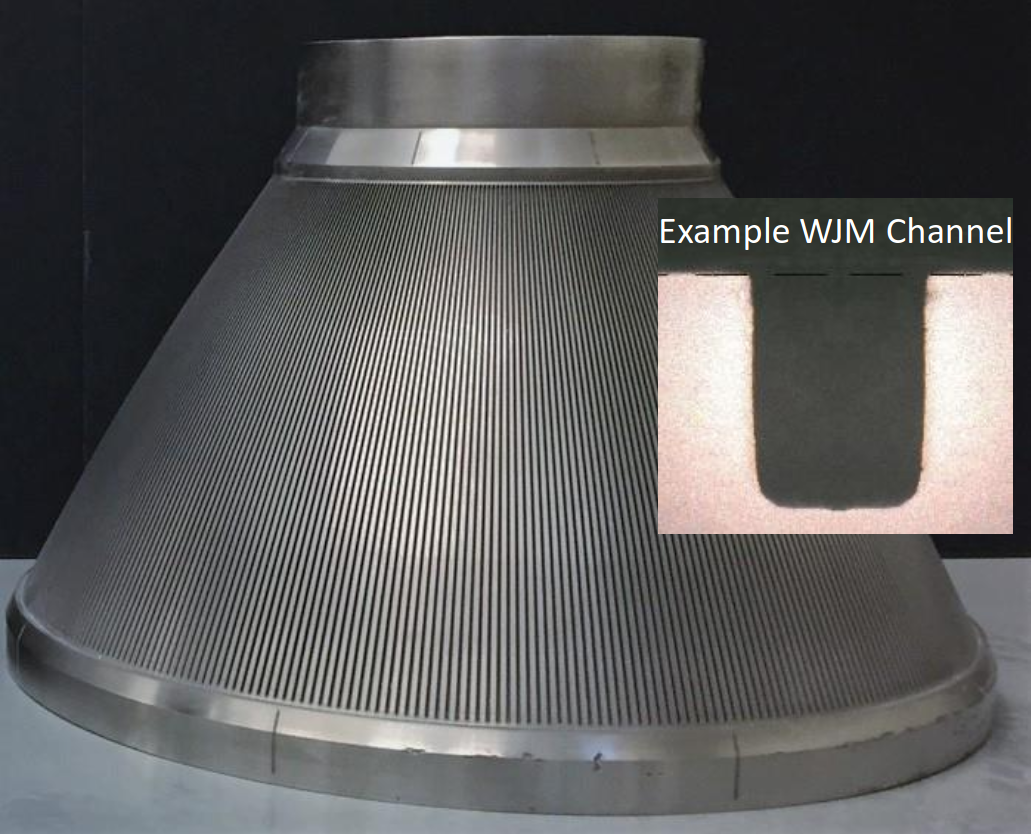
\includegraphics[height=6.3cm]{images/regen_NASA.png}};
  \node[anchor=north east, inner sep=0] (C) at (\textwidth,0)
    {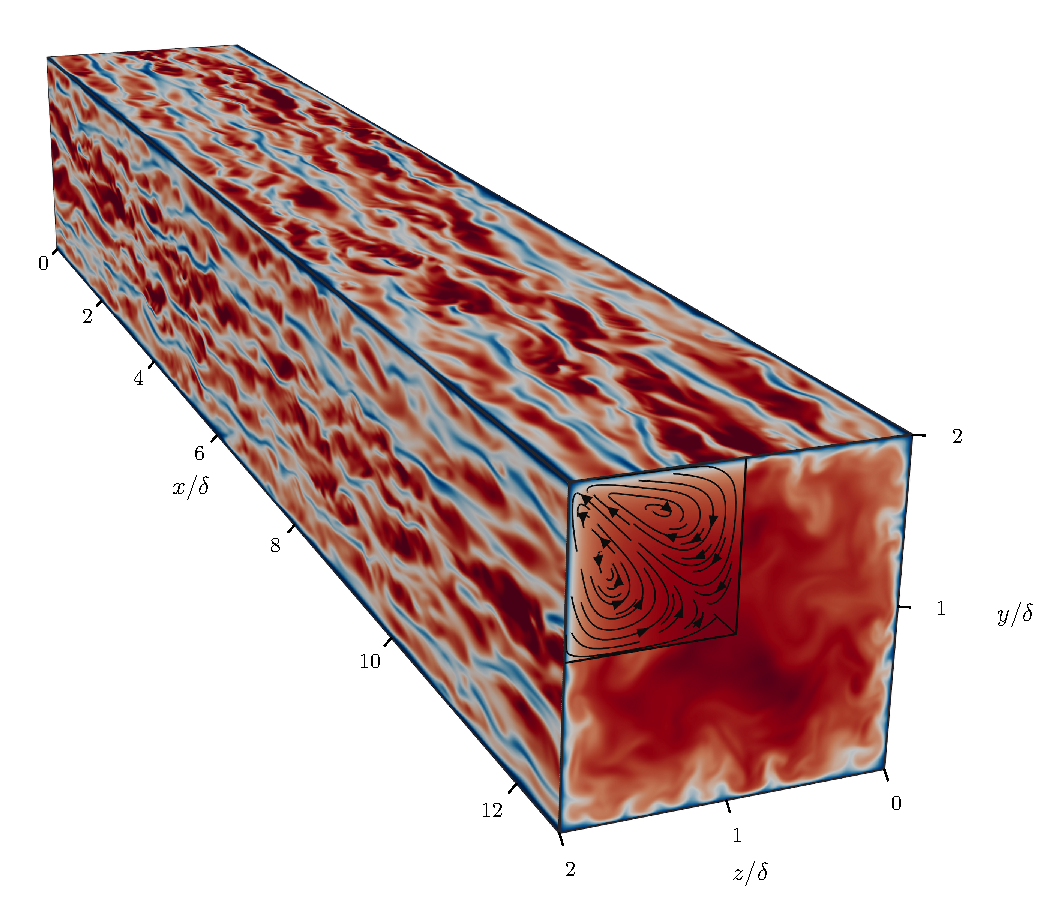
\includegraphics[height=6.3cm]{images/duct_L8.pdf}};
  \node[below=1pt of B] {\small (a)};
  \node[below=1pt of C] {\small (b)};
  \def\Bw{7.788cm}\def\Bh{6.3cm}\def\Cw{7.274cm}\def\Ch{6.3cm}
  \coordinate (I1) at ([xshift=0.639*\Bw, yshift=0.36*\Bh]B.south west);
  \coordinate (I2) at ([xshift=0.985*\Bw, yshift=0.745*\Bh]B.south west);
  \coordinate (K1) at ([xshift=0.515*\Cw, yshift=0.085*\Ch]C.south west);
  \coordinate (K2) at ([xshift=0.870*\Cw, yshift=0.515*\Ch]C.south west);
  \draw[red!80!black, line width=0.8pt] (I1) rectangle (I2);
  \draw[red!80!black, line width=0.8pt] (K1) rectangle (K2);
  \draw[red!80!black, densely dashed, line width=0.6pt] (I2) -- (K1 |- K2);
  \draw[red!80!black, densely dashed, line width=0.6pt] (I1 -| I2) -- (K1);
\end{tikzpicture}
\caption{(a) Coolant channels in a mid-scale Haynes~230 nozzle liner at NASA, with the cross-section of one channel (inset)~\cite{Gradl2019}. 
(b) DNS of turbulent supercritical CO$_2$ flow in a square duct at 1.5 times the critical pressure, with walls hotter than $T_{pb}$ ($Re_b=12\,000$, $Re_\tau\approx300$, ongoing work). It shows instantaneous streamwise velocity on planes at $y^+\approx15$ from the walls and on the cross-section; the outlined quadrant shows the mean streamwise velocity and the streamlines of the secondary flow.}
\label{fig:duct}
\end{figure}


Beyond mean flow behavior, intermittent turbulent events can generate extreme wall-heat-flux fluctuations and localized thermal loads overlooked by conventional mean-based approaches.
Previous studies have characterized extreme wall events primarily in ideal-gas and constant-property turbulence \cite{Hack2021,Zhang2023}, but their underlying mechanisms and predictive precursors under supercritical conditions remain poorly understood.
In my preliminary investigations of turbulent CO$_2$ channel flow, I identified fluctuations exceeding ten times their root-mean-square value, associated with near-wall vortices transporting fluid of contrasting temperatures towards the wall (Figure~\ref{fig:extreme}a,b) [R3].
As suggested by these findings and my preliminary work at Stanford [R2, R3], information-theoretic causal analysis offers a promising approach to identifying the mechanisms and precursors of extreme events \cite{LozanoDuran2020,Massaro2023}.
Such advances could improve the prediction of critical operating conditions and the reliability of thermal systems.

\begin{figure}[t]
\centering
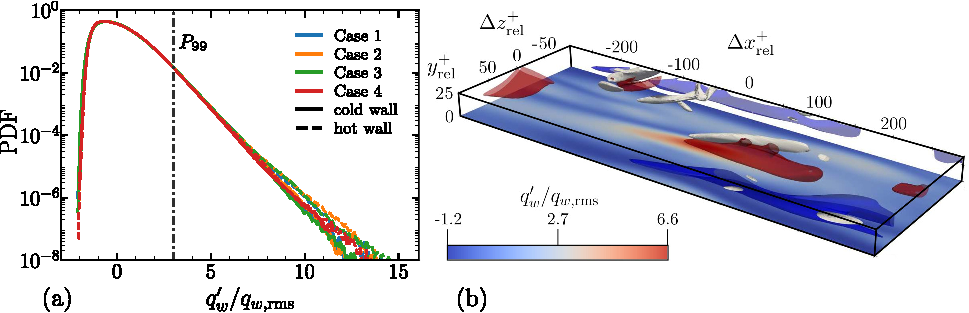
\includegraphics[width=\textwidth]{images/ctr_extreme_events.pdf}
\caption{Extreme wall-heat-flux events in supercritical CO$_2$ channel flow (three transcritical cases and a low-pressure reference) [R3]. (a) Probability density functions of the wall-heat-flux fluctuation normalized by its root-mean-square value, for all cases and both
walls. (b) Instantaneous extreme event at the cold wall of
case~1: wall heat flux (colormap), positive $Q$-criterion isosurfaces (white), and regions of hot (red) and cold (blue) fluid.}
\label{fig:extreme}
\end{figure}

Moreover, addressing these challenges requires increasingly sophisticated computational capabilities.
High-fidelity simulations must resolve strong property gradients, investigate increasingly demanding flow conditions, and capture sufficient statistics of rare events, imposing substantial computational costs.
These requirements motivate the continued development of efficient, scalable numerical methods capable of exploiting modern GPU-based supercomputing architectures.
Building on RHEA-X [J1], advances in real-fluid property evaluation, computational performance, and Lagrangian analysis will support these investigations.
By integrating fundamental flow physics, causal analysis of extreme events, and high-performance scientific computing, the proposed research program aims to advance the understanding and prediction of supercritical turbulent flows, ultimately contributing to more efficient and reliable energy and propulsion technologies.

\subsection{Research lines and objectives}\label{sec:lines}

The program is organized in three research lines, which follow closely the ones specified in the call (Figure~\ref{fig:lines}). 
This section highlights how my research background and experience led to each line, its open problems, and the resulting objectives (O) and expected outcomes.

\begin{figure}[t]
\centering
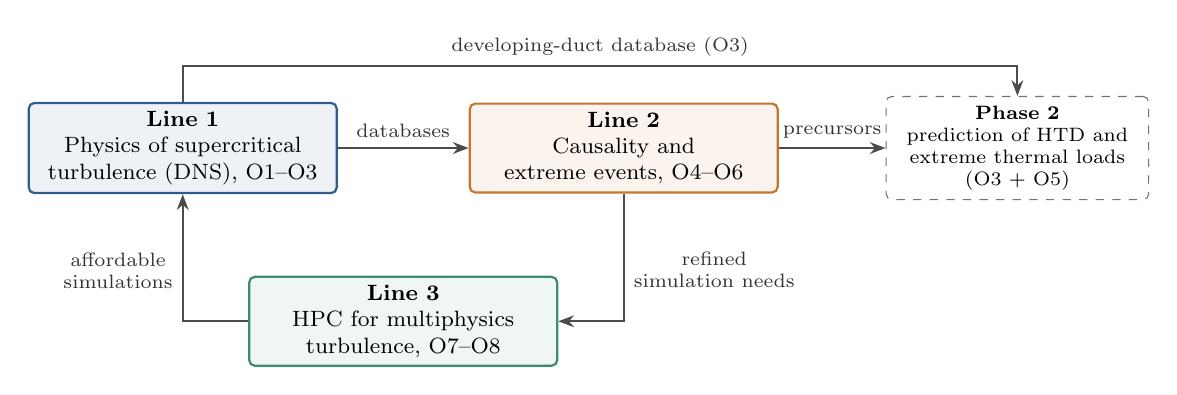
\begin{tikzpicture}[font=\footnotesize,
  box/.style={draw=#1, fill=#1!8, rounded corners=2pt, line width=0.8pt, align=center,
              text width=3.7cm, minimum height=1.05cm, inner sep=3pt},
  arr/.style={-{Stealth[length=2mm]}, line width=0.7pt, black!70},
  lab/.style={font=\scriptsize, align=center, black!80}]
  \definecolor{LA}{HTML}{2F5D8A}\definecolor{LB}{HTML}{C8742B}\definecolor{LC}{HTML}{3C8D6E}
  \node[box=LA] (L1) at (0,0) {\textbf{Line 1}\\ Physics of supercritical\\ turbulence (DNS), O1--O3};
  \node[box=LB] (L2) at (5.6,0) {\textbf{Line 2}\\ Causality and\\ extreme events, O4--O6};
  \node[box=LC] (L3) at (2.8,-2.2) {\textbf{Line 3}\\ HPC for multiphysics\\ turbulence, O7--O8};
  \node[draw=black!55, dashed, rounded corners=2pt, align=center, font=\scriptsize,
        text width=3.1cm, minimum height=1.05cm] (P) at (10.6,0)
        {\textbf{Phase 2}\\ prediction of HTD and\\ extreme thermal loads\\ (O3 + O5)};
  \draw[arr] (L1) -- node[lab, above] {databases} (L2);
  \draw[arr] (L2) -- node[lab, above] {precursors} (P);
  \draw[arr] (L2.south) |- node[lab, pos=0.3, right] {refined\\ simulation needs} (L3.east);
  \draw[arr] (L3.west) -| node[lab, pos=0.7, left] {affordable\\ simulations} (L1.south);
  \draw[arr] (L1.north) |- ++(0,0.45) -| node[lab, pos=0.25, above] {developing-duct database (O3)} (P.north);
\end{tikzpicture}
\caption{Schematic of the scientific connection and dependencies between the three research lines of this program.}
\label{fig:lines}
\end{figure}

\subsubsection{Line 1 -- Physics of supercritical turbulent flows}

My doctoral investigations demonstrated how pseudo-boiling can be exploited to enhance heat transfer and fundamentally modify turbulence in microconfined flows~[J2--J7].
In asymmetrically heated microducts, I showed that pseudo-boiling can trigger turbulence-like regimes under hydrodynamic conditions that remain laminar at low pressure, increasing the hot-wall Nusselt number by approximately $20\times$ with the same imposed temperature difference [J3, J4, J7].
In turbulent square ducts, I demonstrated that secondary-flow intensity can reach 4.6\,\% of the bulk velocity, approximately twice the upper bound reported for canonical ducts.
Moreover, changing the orientation of gravity altered secondary-flow intensity by more than 100\,\% and the hot- and cold-wall Nusselt numbers by up to 28\,\% and 63\,\%, respectively, despite variations below 10\,\% and 3\,\% in bulk and friction Reynolds numbers.
These findings revealed how buoyancy and pseudo-boiling interact to reorganize secondary motions and redistribute momentum, wall shear stress, and turbulent transport [J2, R1, C1].
During my research, I also revisited conventional DNS practices and established refined resolution and minimal-flow-unit guidelines for pseudo-boiling turbulence [J5, J6], demonstrating that grids reproducing first-order statistics within 2\,\% can nevertheless underestimate the intensity and wall proximity of the pseudo-boiling region, with substantial impact on turbulent intensities.

Informed by these contributions, this research line will pursue three complementary investigations, progressing from fundamental transport mechanisms to predictive correlations and the characterization of heat-transfer deterioration (HTD) in increasingly engineering-relevant configurations for space propulsion and thermodynamic cycle technologies:
\begin{enumerate}
	\item \textbf{Thermal transport mechanisms in asymmetrically heated ducts.}
	The first investigation will extend my previous analyses of asymmetrically heated channels and square ducts, where pseudo-boiling interacts with buoyancy and turbulence anisotropy.
	Although the organization of momentum transport and secondary motions has been characterized, the corresponding thermal mechanisms remain less thoroughly understood.
	Using existing DNS databases, I will investigate enthalpy and turbulent heat-flux budgets to quantify how buoyancy, secondary motions, and pseudo-boiling redistribute thermal energy and influence local heat transfer.
	In parallel, attention will be devoted to higher-order statistics and coherent turbulent structures associated with extreme wall-heat-flux events, especially at the heated wall.
	These analyses will establish a comprehensive physical interpretation of heat-transfer modulation and provide reference cases for the causal investigations developed in Line~2.
	
	\item \textbf{Generalized scaling laws and predictive correlations.}
	The second investigation, with simulations already underway (Figure~\ref{fig:duct}b), will examine high-pressure transcritical rectangular ducts with uniform perimeter heating, enabling systematic comparisons with canonical duct flows.
	By varying Reynolds number, thermophysical conditions, and aspect ratio, I will investigate the scaling of skin friction and Nusselt number, alongside momentum and thermal balances.
	Since existing correlations and variable-property transformations may lose accuracy under pseudo-boiling conditions \cite{Modesti2026,Li2025}, these simulations will support their critical assessment and the development of improved physics-based correlations and complementary data-driven models, an effort already initiated in collaboration with Prof.~Xiang Yang (Pennsylvania State University).
	The ambition is to establish broadly applicable predictive relationships that capture the combined influence of Reynolds number, turbulence anisotropy, buoyancy, and thermophysical conditions.
	
	\item \textbf{Heat-transfer deterioration in spatially developing flows.}
	The third investigation will extend the analysis towards spatially developing flows representative of supercritical cooling passages.
	Although previous studies have identified operating conditions associated with HTD, accurately predicting its onset remains challenging, and the underlying physical mechanisms continue to be debated \cite{Nasuti2021,Li2025}.
	Existing correlations can mispredict peak wall temperatures by up to 200~K near the critical pressure, illustrating the limitations of current predictive descriptions \cite{Nasuti2021}.
	I will perform DNS of spatially developing channels and square ducts heated from one side, progressively incorporating more representative heating conditions and cooling-passage geometries.
	These simulations will identify the mechanisms governing HTD onset, including the potentially synergistic influence of buoyancy, secondary motions, and the evolving thermal boundary layer.
	The resulting databases will also provide a demanding assessment of the predictive relationships developed in the second investigation, identifying their limitations and guiding their extension towards deteriorated heat-transfer conditions.
\end{enumerate}
Together, these investigations pursue three complementary scientific objectives:
\begin{itemize}
	\item[\textbf{O1.}] Identify and quantify how pseudo-boiling, buoyancy, and secondary motions govern turbulent heat transfer and extreme wall-heat-flux events in asymmetrically heated ducts relevant to regenerative cooling and energy-conversion systems.
	
	\item[\textbf{O2.}] Establish generalized scaling laws for skin friction and heat transfer in supercritical flows, identifying physically motivated dimensionless parameters that capture the combined effects of Reynolds number and pseudo-boiling to develop improved predictive correlations.
	
	\item[\textbf{O3.}] Elucidate the mechanisms governing HTD onset in spatially developing, asymmetrically heated ducts, quantifying the influence of secondary motions and cooling-passage geometry on thermal deterioration.
\end{itemize}
The program will deliver openly accessible, highly curated DNS databases spanning different heating conditions (both asymmetric and perimeter heating), Reynolds-number effects, and spatially developing flows exhibiting HTD, establishing reference benchmarks for the research community.
These will underpin generalized scaling laws and improved skin-friction and Nusselt-number correlations, including the identification of new dimensionless parameters to potentially capture the combined effects of Reynolds number, turbulence anisotropy in rectangular ducts, buoyancy, and supercritical thermodynamic conditions.
The research will also seek to establish a comprehensive physical understanding of HTD onset, identifying its governing mechanisms and developing predictive criteria for its occurrence.
Ultimately, these contributions will provide a high-fidelity foundation for validating and improving lower-fidelity computational fluid dynamics (CFD) approaches (RANS and LES) and extending predictive capabilities towards increasingly complex, engineering-relevant geometries and operating conditions.
\NEW{Where feasible, the correlations and HTD criteria developed in this line could also be compared with experiments, potentially through collaborations within GReCEF and the UPC (Section~\ref{sec:mobility}).}

Depending on funding availability, a complementary investigation of supercritical jets and mixing layers may also be pursued.
Previous investigations have shown that pseudo-boiling can substantially modify shear-layer instability and jet development \cite{Lapenna2019,SharanBellan2021}, yet its influence on turbulent interfaces and entrainment remains poorly characterized.
Building on the existing capabilities of RHEA-X [J1], I will investigate interactions between liquid-like and gas-like streams of the same fluid, isolating pseudo-boiling effects from the complexities of multicomponent mixing and advancing the understanding of turbulent entrainment relevant to high-pressure injection and film cooling.
In the longer term, this framework could be extended to multispecies mixing and transcritical atomization, addressing the coupled thermodynamic and interfacial phenomena encountered in high-pressure propulsion systems \cite{JofreUrzay2021}.

\subsubsection{Line 2 -- Causality and extreme events in multiphysics turbulence}

Extreme events in turbulent flows, from severe storms and floods to localized thermal loads in engineering systems, often have consequences far beyond those suggested by average conditions.
Rare fluctuations can dominate critical transport processes and impose loads that conventional mean and root-mean-square statistics fail to capture~\cite{Guerrero2020}.
Understanding the mechanisms preceding such events and whether they can be anticipated is therefore essential for improving prediction and reliability.
Conventional approaches such as conditional averaging characterize the turbulent structures around extreme events but do not establish their causal relationships \cite{Hack2021,Zhang2023}.
During the 2026 CTR Summer Program, I initiated an alternative approach combining event-conditioned Eulerian statistics, Lagrangian tracking, and transfer entropy to investigate extreme wall-heat-flux events in supercritical CO$_2$ turbulence [R2, R3].
These investigations revealed a sequence of near-wall turbulent motions preceding extreme thermal events and identified candidate precursors carrying predictive information.
Building on these findings, this research line will develop through two complementary activities:
\begin{enumerate}
	\item \textbf{Causality and prediction of extreme events in supercritical turbulence.}
	This investigation (under-development) combines the formalization of a non-stationary Lagrangian information-theoretic framework with its application to extreme wall-heat-flux events.
	Extending the preliminary transfer-entropy analyses [R2, R3], the primary approach to be tested will be the incorporation of multivariate decompositions of unique, redundant, and synergistic contributions \cite{MartinezSanchez2024}.
	Its application to the existing databases will establish how pseudo-boiling influences extreme thermal events and their precursors.
	This work should have reached a mature stage by the start of the Lector appointment to subsequently be applied to the developing-flow databases of Line~1 to identify the causal precursors of HTD and establish predictive criteria for its onset.
	
	\item \textbf{Generalization of the causal analysis approach to multiphysics turbulent systems.}
	The framework will be applied to physically distinct problems.
	The first application will address microplastic--biogenic particle collisions and aggregation in ocean turbulence, drawing on my summer 2027 research stay with Prof.~Mona Rahmani at the University of British Columbia.
	A subsequent research stay at the Universit\`a del Salento with Prof.~Mario Di Renzo and Prof.~Donatella Passiatore will support its extension to extreme thermal events in hypersonic boundary layers.
	A prospective third international stay at the California Institute of Technology, hosted by Prof.~Adrián Lozano-Durán, will provide additional opportunities to consolidate and validate the methodology across turbulent flow regimes (see Section~\ref{sec:mobility}).
\end{enumerate}
The natural follow-up scientific objectives are:
\begin{itemize}
	\item[\textbf{O4.}] Develop and validate a non-stationary Lagrangian information-theoretic framework for assessing causal relationships and identifying predictive precursors of rare turbulent events.
	\item[\textbf{O5.}] Identify the causal mechanisms and precursors of extreme events in supercritical turbulence and evaluate their predictive value across thermophysical and buoyancy regimes.
	\item[\textbf{O6.}] Demonstrate the framework's generality through applications to particle interactions in ocean turbulence and extreme thermal events in compressible and hypersonic flows.
\end{itemize}
The expected deliverables include an open-source, validated Lagrangian causality framework, benchmark cases for rare-event analysis, and physically interpretable predictive indicators of extreme wall-heat-flux events and HTD onset.
Its testing across different multiphysics turbulent flows will establish a high-impact transferable methodology for investigating and anticipating extreme events.

\subsubsection{Line 3 -- High-performance computing for high-fidelity simulation of complex turbulent flows}

RHEA-X [J1] is the computational code for the simulations in Lines~1 and~2. 
Improving it is a natural next step as these investigations move towards larger and more complex simulations and research goals. 
Additionally, this line of work also serves a broader goal of establishing RHEA-X as a reference tool for high-fidelity CFD by improving its performance while maintaining reproducibility, and enabling researchers to add physical models and diagnostics through documented interfaces that reuse optimized GPU routines.
I co-developed RHEA-X, the successor to the open-source RHEA solver~\cite{RHEASoftware}, and led its port to distributed GPUs. 
The port retains a common C++ source for CPU and GPU (OpenACC~\cite{OpenACC}) execution, keeps flow fields resident on the device, and uses GPU-aware MPI for halo exchanges. 
Benchmarks on different supercomputers (such as MareNostrum~5 at the Barcelona Supercomputing Center (BSC)~\cite{BSC} and the Netherlands' national supercomputer Snellius~\cite{Snellius}) demonstrated speedups of up to $70\times$ over CPU execution and strong-scaling efficiencies of up to $97\,\%$ on as many as 64 GPUs [J1]. 
Extending this foundation, I plan to advance the following topics:
\begin{enumerate}
	\item \textbf{Systematic kernel optimization across CPUs and GPUs.}
	I will benchmark different optimization strategies such as optimized data layout, cache reuse, kernel fusion and splitting, and asynchronous computation on representative DNS workloads. 
	Comparisons across different architectures and paradigms (such as SYCL~\cite{SYCL}) will establish which optimizations transfer across architectures and which depend on the hardware or workload. 
	I will document their effects on runtime, memory use, scaling and agreement in flow statistics, with reproducible cases that other CFD developers can use to test the same choices.
	
	\item \textbf{Reliable substitution of costly physical models with surrogates.}
	I will establish a procedure to determine when a surrogate can replace a computationally demanding model. 
	The first demonstration builds on [R4], where I am contributing to a surrogate model trained on CoolProp data~\cite{CoolProp2014} to replace selected property evaluations based on the Peng--Robinson equation of state~\cite{PengRobinson1976}. 
	Additionally, I will quantify the gains in runtime and device memory alongside the errors in thermophysical properties and their gradients near pseudo-boiling.
	
	\item \textbf{Guidelines for integrating new physical models and diagnostics.}
	I plan to develop documented hybrid C++-OpenACC interfaces, implementation examples and verification cases that let contributors reuse the solver's accelerated capabilities when testing their own ``plug-ins''. 
	The guidelines will show how to implement a module, verify its results on CPUs and GPUs, and measure its cost in a full DNS. 
\end{enumerate}
The aim of these contributions is to make the code a general well-established platform for high-fidelity CFD for academic and research purposes that enables a straightforward implementation of additional physical models in a unified reproducible platform that seamlessly leverages the advent of GPU-accelerated architectures (from laptops to supercomputers), a clear void in the current CFD community. 
The optimization benchmarks will guide implementation choices, the surrogate-model approach will establish cheaper models leveraging highly reliable databases, and the integration guidelines will make both accessible to potential contributors. 
This should also support longer-term investigations of high-speed supercritical flows, including shock interactions and multicomponent mixing, with reacting flows and finite-rate chemistry as subsequent extensions.
Therefore, two main objectives are established in this research line:
\begin{itemize}
	\item[\textbf{O7.}] Establish reproducible methods for optimizing DNS kernels across accelerated HPC architectures and for validating GPU-friendly surrogate-models.
	\item[\textbf{O8.}] Enable researchers to seamlessly integrate and verify GPU-capable models through documented interfaces, promoting scientific collaboration.
\end{itemize}

The deliverables will be versioned open-source releases of RHEA-X, reproducible benchmarks, and implementation guidelines with verified examples. 
These resources will support simulations in Lines~1 and~2, and the generation of documented datasets for physical analysis and data-driven modeling. 
The feasibility of this line also builds on six previous successful competitive supercomputing allocations (described in the HAP), two MareNostrum hackathons, ongoing collaboration with Xavier Álvarez-Farré (SURF), and technical exchanges with Lucas Gasparino (BSC) and Filippo Spiga (NVIDIA). 
The shared code and benchmarks will also support joint development and validation during the planned international research stays (Section~\ref{sec:mobility}).
Besides participating in further hackathons and continuing to apply for national allocations through the Spanish Supercomputing Network (RES), I plan to leverage this experience to apply for EuroHPC allocations, with the aim of scaling RHEA-X towards exascale performance.
Quantum computing also sparks my curiosity, and its feasibility for CFD, even as a partial offload, is a potential topic to explore in the long term~\cite{Bharadwaj2023}.

\subsection{Work plan, timeline and risks}\label{sec:workplan}

The plan covers six years, from September 2027 to August 2033, with Year~1 corresponding to the academic year 2027--28. 
It consists of two phases.
\textbf{Phase~1 (2027--30)} delivers the databases, the generalized causal framework and the optimized solver, while \textbf{Phase~2 (2030--33)} builds on them to provide predictive criteria for HTD onset and extreme events, engineering correlations and, if funding allows, the study of free shear flows.
I intend to develop this program within GReCEF (\emph{Grup de Recerca en Ci\`encia i Enginyeria de Fluids}, Fluid Science and Engineering Research Group)~\cite{GReCEF}, an established research group of the UPC Department of Fluid Mechanics. 
The proposed work can be divided into four work packages (WPs), each composed of tasks (T) with a specific goal.

\begin{enumerate}[label=\textbf{WP\arabic*}, leftmargin=*]
	\item \textbf{Physics of supercritical turbulence and DNS database development (Line~1).}
	\begin{enumerate}[label=T1.\arabic*, leftmargin=*, nosep]
		\item Finalize the heat-transfer analysis of existing asymmetrically heated duct-flow databases.
		\item Develop comprehensive DNS databases of (i) uniformly perimeter-heated rectangular ducts and (ii) spatially developing, asymmetrically heated rectangular ducts.
		\item Establish generalized friction and heat-transfer scaling laws, including physics-based correlations and complementary data-driven models developed with Penn State.
		\item Identify the mechanisms governing HTD onset and recovery, and assess and extend predictive correlations to deteriorated heat-transfer regimes.
		\item Subject to funding and computational resources, extend the investigation to pseudo-boiling effects on entrainment in free shear flows.
	\end{enumerate}
  \item \textbf{Causality and prediction of extreme events (Line~2).}
  \begin{enumerate}[label=T2.\arabic*, leftmargin=*, nosep]
    \item Mathematically formalize, validate and release the Lagrangian causality framework.
    \item Identify the precursors of extreme wall-heat-flux events in developed flows.
    \item Generalize the framework to other flows (through the stays at UBC, Salento and Caltech).
    \item Deliver validated criteria to predict HTD onset in developing flows.
  \end{enumerate}
  \item \textbf{High-performance computing (Line~3).}
  \begin{enumerate}[label=T3.\arabic*, leftmargin=*, nosep]
    \item Optimize the solver kernels and integrate validated surrogate models.
    \item Release documented interfaces for on-device Lagrangian tracking and event detection.
    \item Obtain EuroHPC allocations and scale the solver towards exascale.
  \end{enumerate}
  \item \textbf{Mobility, team and funding (refer to Sections~\ref{sec:resources} and~\ref{sec:mobility}).}
  \begin{enumerate}[label=T4.\arabic*, leftmargin=*, nosep]
    \item Complete the international research stays (see Section~\ref{sec:mobility}).
    \item Co-direct a first doctoral thesis, associated with WP1.
    \item Direct a second doctoral thesis, associated with WP2 or WP3.
    \item Submit a first national proposal on causality and extreme events as principal investigator (PI) or co-PI and, if funded, execute it.
    \item Prepare an ERC Starting Grant proposal or a follow-up national proposal (long-term).
  \end{enumerate}
\end{enumerate}

Figure~\ref{fig:timeline} distributes these tasks over three stages of increasing independence: establishment (Phase~1), followed by development and consolidation, which together form Phase~2 (see Figure~\ref{fig:lines}).

The \textbf{establishment stage (2027--30)} builds the foundations of this research independence. 
I will integrate GReCEF through its ongoing projects, as a member of the research team, and co-direct the first doctoral student within the first two years, after which I plan to submit the first project proposal as PI. 
Through this participation, and supported by initial funding (see Section~\ref{sec:resources}) starting in 2027--28, I will continue publishing as first author through the ongoing work and collaborations (CTR and UBC) on high-pressure transcritical flows, causality and extreme events [R1, R3]. 
In spring 2028, I will spend three months at Universit\`a del Salento, with teaching arranged with the Department. 
By summer 2029, the first database (T1.2), the causality code (T2.1) and the optimized solver (T3.1) will be ready for the developing-flow simulations. 
Meanwhile, I will apply for funding for the Caltech stay by the beginning of 2029 (see Section~\ref{sec:mobility}). 
This stay, from September 2029 to February 2030, will complete the mobility required for accreditation. 
These results and collaborations will support my first national proposal, to be submitted in late 2029 as sole PI or as co-PI with another early-career researcher.

The \textbf{development stage (2030--32)} marks the transition from contributing to projects to leading them. 
In autumn 2030, with the teaching and mobility requirements completed, I will apply for the AQU \textit{Acreditació de Recerca} (research accreditation). 
If the national proposal described in Section~\ref{sec:resources} is funded, this first independent (or shared) project will start in September 2030 and support a relatively small team of two doctoral students and master's students. 
The developing-flow database (T1.2) will enable the first criteria for HTD onset (T2.4) in 2031--32. That same year, the second doctoral thesis will start under my direction, and the preparation of the ERC proposal will begin.

The \textbf{consolidation stage (2032--33)} builds on these results to establish my research leadership. 
I will submit the ERC Starting Grant proposal in autumn 2032 and/or a follow-up national proposal in late 2032, so that the team and the second thesis continue after the first project ends in August 2033. 
By then, the research and teaching record should support my stabilization as \textit{Professor Agregat}.

\begin{figure}[!htb]
\centering
\definecolor{GLineA}{HTML}{2F5D8A}%
\definecolor{GLineB}{HTML}{C8742B}%
\definecolor{GLineC}{HTML}{3C8D6E}%
\definecolor{GCross}{HTML}{8C96A0}%
\begin{ganttchart}[
    hgrid={*1{black!10}},
    vgrid={*3{black!10, dashed}, *1{black!35}},
    x unit=0.48cm, y unit title=0.5cm, y unit chart=0.44cm,
    time slot format=simple,
    canvas/.append style={draw=black!35, line width=0.4pt},
    title/.append style={draw=black!35, fill=MSBlue!12},
    title label font=\scriptsize\bfseries\color{MSBlue},
    title height=1,
    bar height=0.5, bar top shift=0.25,
    bar/.append style={draw=none, rounded corners=1.5pt},
    bar label font=\scriptsize,
    bar label node/.append style={align=right}
  ]{1}{24}
  \gantttitle{Establishment}{12}\gantttitle{Development}{8}\gantttitle{Consolidation}{4}\\
  \gantttitle{2027--28}{4}\gantttitle{2028--29}{4}\gantttitle{2029--30}{4}\gantttitle{2030--31}{4}\gantttitle{2031--32}{4}\gantttitle{2032--33}{4}\\
  \ganttbar[bar/.append style={fill=GLineA}]{T1.1 Heat-transfer analysis}{1}{8}\\
  \ganttbar[bar/.append style={fill=GLineA}]{T1.2 DNS databases}{1}{16}\\
  \ganttbar[bar/.append style={fill=GLineA}]{T1.3 Scaling and correlations}{1}{12}\\
  \ganttbar[bar/.append style={fill=GLineA}]{T1.4 HTD onset and recovery}{9}{20}\\
  \ganttbar[bar/.append style={fill=GLineA!25, draw=GLineA, dashed}]{T1.5 Free shear flows}{17}{24}\ganttnewline[black!45]
  \ganttbar[bar/.append style={fill=GLineB}]{T2.1 Framework validation}{1}{8}\\
  \ganttbar[bar/.append style={fill=GLineB}]{T2.2 Extreme-event precursors}{1}{12}\\
  \ganttbar[bar/.append style={fill=GLineB}]{T2.3 Generalization}{1}{12}\\
  \ganttbar[bar/.append style={fill=GLineB}]{T2.4 Prediction of HTD onset}{13}{24}\ganttnewline[black!45]
  \ganttbar[bar/.append style={fill=GLineC}]{T3.1 Kernels and surrogates}{1}{8}\\
  \ganttbar[bar/.append style={fill=GLineC}]{T3.2 Interfaces and tracking}{5}{12}\\
  \ganttbar[bar/.append style={fill=GLineC}]{T3.3 Scaling towards exascale}{5}{24}\ganttnewline[black!45]
  \ganttbar[bar/.append style={fill=GCross}]{T4.1 Stays (Salento, Caltech)}{3}{3}%
  \ganttbar[inline, bar/.append style={fill=GCross!40, draw=GCross, dashed}]{}{9}{10}\\
  \ganttbar[bar/.append style={fill=GCross}]{T4.2 Co-direction (thesis 1)}{3}{18}\\
  \ganttbar[bar/.append style={fill=GCross!40, draw=GCross, dashed}]{T4.3 Direction (thesis 2)}{17}{24}\\
  \ganttbar[bar/.append style={fill=GCross}]{T4.4 National proposal and project}{1}{10}%
  \ganttbar[inline, bar/.append style={fill=GCross!40, draw=GCross, dashed}]{}{13}{24}\\
  \ganttbar[bar/.append style={fill=GCross}]{T4.5 ERC or follow-up proposal}{17}{22}
\end{ganttchart}
\caption{Indicative timeline of the different work packages and tasks. Dashed bars depend on funding.}
\label{fig:timeline}
\end{figure}

\subsection{Risk management} 

The research plan will be periodically reassessed against funding availability, eligibility for competitive calls, doctoral recruitment, computational resources, and progress towards scientific and accreditation milestones.
Delays or unsuccessful applications will be mitigated by prioritizing ongoing projects, existing DNS databases, alternative funding and recruitment schemes, and adjustments to the timing and scope of individual tasks.
Methodological uncertainties and international mobility constraints will be addressed through alternative analysis strategies, established collaborations, and flexible scheduling, preserving the programme's core scientific objectives.

%%%%%%%% CARLOS IS HERE %%%%%%%%%%%%%

\newpage
\subsection{Funding and resources}\label{sec:resources}


%\paragraph{Independent output before the first project.} 
Until a project as principal investigator starts (autumn 2030 at the earliest), the research would build on the existing databases, the RHEA-X solver and yearly competitive computing allocations. 
Collaboration and integration of ongoing projects of GReCEF with similar research interests would also be prioritized.
During the first three years of the contract (Y1--Y3) I will keep publishing as first and corresponding author in the lines I lead: wall-bounded supercritical fluid flows causality manuscripts [R1--R3], the causal framework (T2.1) and the joint work of the UBC, Salento and Caltech stays, with a target of about two journal articles per year. 
This record of independent output is the basis of the first proposal as principal investigator and, later, of the ERC Starting Grant proposal.

\subsubsection{Funding strategy}
%\paragraph{Funding strategy.} 
The Lector position provides the institutional framework to
apply for competitive funding as principal investigator. 
The funding applications below are planned, subject to eligibility and successful evaluation, and each one supports specific objectives of Section~\ref{sec:research}.
\begin{itemize}
  \item \textbf{Initial funding (2027--29).} The UPC ALECTORS program for newly appointed Lector staff, subject to the call conditions, to start WP1--WP3; participation in the ongoing projects of GReCEF, as a member of the research team for the period prior to my own application as PI (late 2029). 
  I would co-direct doctoral student~1, funded by these projects or by competitive predoctoral grants (AGAUR FI Joan Or\'o, FPU of the Ministry and UPC predoctoral grants).
  
  \item \textbf{Independent national funding (2027--33).} An AEI \emph{Proyecto de Generaci\'on de Conocimiento}, Tipo~A, prepared during the establishment stage and submitted in late 2029 (Y3) as sole PI, co-PI or research team member, depending on eligibility. 
  The AEI Tipo-A allows for two early-career PIs with equal standing~\cite{AEI2025}. 
  The objective is to secure a three-year project (2030-2033) on HTD in developing supercritical flows and the causal prediction of extreme heat-transfer events. 
  An associated predoctoral contract (FPI) for doctoral student~2 will be requested where the call allows it. 
  AGAUR \emph{Doctorats Industrials} with companies in the energy and space sectors will also be considered for transfer of discovered concepts to realistic engineering systems.
  
  \item \textbf{Research development (2030--33).} Execution of the first independent or shared project, if funded, and complementary collaborative funding where compatible with it: Horizon Europe Cluster~5 (Climate, Energy and Mobility) consortia, \emph{Redes de Investigaci\'on}   with Spanish groups on supercritical and compressible flows, and Marie Sk\l{}odowska-Curie Postdoctoral Fellowships and Doctoral Networks hosted at the UPC.
  
  \item \textbf{Major international funding (2031--33).} Building on the experience from \NEW{the success} of the national project, I would make the \NEW{necessary} preparations for an ERC Starting Grant proposal to submit toward the concluding stages of my appointment as \textit{\NEW{Professor} Lector}. This would ideally be prepared in 2031--32 and submitted in 2032, subject to the eligibility of the corresponding call; and a follow-up national proposal to ensure the continuity of the doctoral projects.
\end{itemize}

\subsubsection{Long-term direction}

By the end of the contract, and looking further in the long-term perspective, the program aims to \NEW{predict} the consequences of strong property variations in engineering flows: both the transport and mixing enhancement that the applications seek and the HTD and extreme thermal loads that limit them, in regenerative cooling channels and sCO$_2$ heat exchangers~\cite{Pizzarelli2018,Ahn2015}. 
The same capabilities lead naturally to high-speed aerothermodynamics, where extreme wall heat fluxes, large property variations and thermochemical effects coexist~\cite{Urzay2018,DiRenzoUrzay2021,Passiatore2022}. 
This extension continues my work on variable-property turbulence, extreme thermal events and GPU-accelerated high-fidelity CFD. 
It starts with T2.3 at the Universit\`a del Salento, whose hosts have studied hypersonic boundary layers~\cite{DiRenzoUrzay2021,Passiatore2022}, is consolidated during the Caltech stay, and is in line with the department's priority on compressible flows. 
Extending RHEA-X to high-speed supercritical flows, with shock interactions and multicomponent mixing, is a longer-term development (Line~3).
Therefore, the ERC Starting Grant is placed deliberately at the end of the contract. 
By then, the proposal can build on the results of the first independent project, experience managing competitive funding, doctoral supervision, an independent publication record, and the collaborations established at UBC, Salento and Caltech. 
Its scientific question will go substantially beyond the national project: from understanding supercritical turbulence and extreme events to their causal prediction and control in real-fluid and high-speed flows.
\NEW{The proposal would also include an experimental component, developed in collaboration with GReCEF, to test whether the precursors and criteria identified through simulations can anticipate HTD through measurable quantities, such as wall temperature.}

\subsubsection{Engineering transfer} 
From Phase~2 and beyond the contract, the program will carry its results to engineering design in two steps.
\begin{enumerate}
	\item The DNS databases would calibrate and validate the models that engineering tools need. In particular correlations and transformations (O2) would be tuned, as well as turbulent Prandtl number and wall models for RANS and LES, and data-driven models of velocity and temperature profiles. The real-fluid property surrogate models or other developed methods in RHEA-X of Line~3 [R4] could \NEW{potentially} be coupled to OpenFOAM, so that RANS and LES of real cooling passages and heat exchangers use the thermophysics validated by DNS.
	
	\item \NEW{These} tools will be applied to real industrial applications such as: regeneratively cooled channels produced by additive manufacturing, including wall roughness and conjugate heat transfer (Figures~\ref{fig:regen}a and~\ref{fig:duct}a); 
	sCO$_2$ Brayton cycles, whose precoolers, recuperators and compressor inlet operate near the pseudo-critical point~\cite{Ahn2015}; 
	\NEW{transcritical} CO$_2$ heat pumps, whose gas coolers operate across pseudo-boiling; and \NEW{supercritical} organic Rankine cycles for waste-heat recovery. 
\end{enumerate}
Waste heat accounts for more than half of the global primary energy~\cite{Markides2025}, and the working fluids of these cycles are changing, highlighting the need for research and development in such technologies. The EU F-gas Regulation phases out HFCs by 2050~\cite{FGas2024}, and the proposed EU restriction of PFAS also covers most HFO working fluids~\cite{ECHA2025}. 
Additionally, drawing from research line~2, design margins that account for extreme events could be established, through probabilistic limits on the wall temperature and precursor-based monitoring.
The majority of these activities could also be carried out through industrial doctorates and contracts with companies in the energy and space sectors.


\subsubsection{Computing resources} 
I plan on applying yearly to the RES calls (MareNostrum~5, BSC) and, from year~2, to the EuroHPC JU \emph{Regular} and \emph{Extreme Scale} calls, which give access to pre-exascale and exascale systems. 
The collaboration with UBC also leverages access to Canadian
national systems through the Digital Research Alliance of Canada, as in the RAC-2026 allocation (See HAP). 
This builds on six national and international competitive allocations in 2023--2026.

\subsubsection{Software and data} 
RHEA-X [J1] (open source, MPI + OpenACC) is the core solver of WP1--WP3. 
If highly complex engineering applications are pursued, well-established open-source RANS and LES software could also be used, such as OpenFOAM~\cite{Weller1998} and SU2~\cite{Economon2016}. %, the last of which also supports non-ideal compressible flows~\cite{Pini2017}.
These would build on the DNS databases established in WP1, using them to tune the model parameters and to validate the resulting predictions.
Post-processing and analysis uses Python, Paraview, the thermophysical surrogate software [R4],  CoolProp~\cite{CoolProp2014} and others. 
Databases should be published in open repositories (Zenodo, Figshare+, BLASTNet [D1]).


\subsection{Team, collaborations and dissemination}\label{sec:mobility}\label{sec:dissemination}

\subsubsection{Doctoral supervision and team}
Teaching at the EEBE allows identifying motivated students early, and bachelor's and master's theses will also be the entry point to the research lines. 
I currently tutor a curricular internship on extreme events in turbulent flows and co-supervised a bachelor's thesis on supercritical duct flow. 
I aim to supervise two 3-4 year doctoral theses during the contract: the first as co-director, within the ongoing projects of GReCEF, and the second as director, linked to my first national project, with co-supervision where it adds expertise. 
Both will be financed through the specific competitive project or predoctoral grants, and their topics contribute directly to the objectives of Section~\ref{sec:research}:
\begin{enumerate}
  \item \textbf{Doctoral thesis 1, co-directed: Predicting the onset of heat-transfer \NEW{deterioration} in supercritical fluid turbulence} (WP1). Funding: ongoing projects of GReCEF, or AGAUR FI Joan Or\'o, FPU and UPC predoctoral grants, subject to the requirements of the doctoral program.
  \item \textbf{Doctoral thesis 2: Causality in extreme heat-transfer events in supercritical fluid turbulence.} Funding: FPI contract associated with the national project, or the next FI and FPU calls.
\end{enumerate}
Together with master's students they form the small team that executes the independent project.
Potential \NEW{bachelor's and master's thesis} topics (TFG \& TFM respectively) are presented in Section~\ref{sec:theses}.

\subsubsection{Ongoing collaborations}
The following collaborations are already active and will continue through shared data, method and codes, regular meetings, co-supervision of students and joint publications; some of them are reinforced by the research stays described in Section~\ref{sec:mobility}.
\begin{itemize}
  \item \textbf{The Pennsylvania State University (USA)}, Prof.\ X.\ Yang: compact neural networks
  for wall-normal profiles, trained on our supercritical-flow databases.
  \item \textbf{CTR, Stanford University (USA)},
  \href{https://me.stanford.edu/people/sanjiva-lele}{Prof.\ S.\ Lele} and his research team, including   A.\ Chandra: a strong international collaboration on non-stationary transfer entropy for extreme wall-heat-flux events in supercritical fluids, building on the joint work with A.\ Chandra in the 2026 CTR Summer Program.
  \item \textbf{Caltech and MIT (USA)}, Prof.\ A.\ Lozano-Dur\'an and \'A.\ Mart\'inez-S\'anchez:   causality and Lagrangian information-theoretic frameworks for turbulence (research stay at Caltech in 2029--30).
  \item \textbf{Stanford University (USA)}, group of Prof.\ M.\ Ihme: contribution of our databases to the BLASTNet machine-learning dataset [D1].
  \item \textbf{University of British Columbia (Canada)}, Prof.\ M.\ Rahmani: causality in ocean turbulence and aggregation of microplastics, already active through the RAC-2026 GPU allocation and to be extended during the \NEW{scheduled} research stay at UBC in \NEW{2027.}
  \item \textbf{Universit\`a del Salento (Italy)}, Prof.\ M.\ Di Renzo and Prof.\ D.\ Passiatore:
  extreme wall-heat-flux events in hypersonic turbulent compression corner (scheduled research stay in 2028).
  \item \textbf{Instituto Superior T\'ecnico, Lisbon (Portugal)}, Prof.\ C.\ B.\ da Silva
  (prospective): turbulent/non-turbulent and turbulent/turbulent interfaces in flows with
  variable properties (depending on funding and time).
  \item \textbf{SURF (the Netherlands)}, X.\ \'Alvarez-Farr\'e: ongoing collaboration on RHEA-X,
  complemented by technical exchanges with F.\ Spiga (NVIDIA).
  \item \textbf{Local partners:} the Institut de Ci\`encies del Mar (ICM-CSIC), on microplastics and biofilms (prospective), and the Barcelona Supercomputing Center, through the BSC hackathons and technical exchanges with L.\ Gasparino (O7).
\end{itemize}

I also aim to build collaborations within the UPC that
complement the research program.
Within GReCEF, J.\ Calafell develops data-driven wall models with graph neural networks, \NEW{and we could collaborate} on machine-learning models trained on the DNS databases (O2) and on wall-modeled LES for the engineering transfer.
Other potential collaborations are J. Casals-Terr\'e (Department of Mechanical Engineering) and M. Jofre (Department of Network Engineering), co-authors of the data-informed analysis of experiments on microconfined transcritical turbulence [J7].
\NEW{With them and within GReCEF, I hope to collaborate on experiments that build on the group's previous work in high-pressure microfluidics~\cite{Hurtan2025}. My simulations would inform the design and measurement requirements of these experiments, which would in turn provide validation data for the conditions they can access.}

\subsubsection{Planned mobility}

Three research stays, of up to 12 months in total, develop the research lines with these groups
and cover the nine months of postdoctoral mobility required for the AQU research
accreditation~\cite{AQU2025}, whose other requirements are given in Section~\ref{sec:targets}.
This mobility is a necessary step in the academic career: the Organic Law of the University System
(LOSU) makes activity at institutions other than that of the doctorate a condition for
accreditation as permanent faculty (arts.~69.1 and 85.3)~\cite{LOSU2023}. It should therefore be
both allowed and promoted. The LOSU recognizes mobility as a right of academic staff (art.~66.1)
and limits the teaching of Lectors to 180 hours per year, precisely so that it remains compatible
with the research needed for their accreditation (art.~78.c)~\cite{LOSU2023}. In turn, the Spanish
Science Law requires public research institutions to promote mobility (art.~17.1)~\cite{LCTI2011},
and the UPC Statutes commit the University to facilitate it as part of the professional development
of its staff (art.~184)~\cite{UPCStatutes2025}. Within this framework, I will agree each stay in
advance with the Department of Fluid Mechanics, counting on its authorization and on its support to
concentrate my teaching in the other semester, so that mobility does not compromise my teaching
commitments.
\begin{itemize}
  \item \textbf{University of British Columbia (Canada), summer 2027, 3 months, before the
  contract.} Host: \href{https://chbe.ubc.ca/mona-rahmani/}{Prof.\ Mona Rahmani}. Lagrangian
  causality applied to the aggregation of microplastics in ocean turbulence (Mitacs Globalink
  Research Award, \NEW{application under evaluation}; T2.3).
  
  \item \textbf{Universit\`a del Salento (Italy), second semester of 2027--28 (Y1), 3 months.} Hosts:
  \href{https://www.unisalento.it/scheda-utente/-/people/mario.direnzo}{Prof.\ Mario Di Renzo}
  and \href{https://www.unisalento.it/scheda-utente/-/people/donatella.passiatore}{Prof.\
  Donatella Passiatore}. Extreme wall heat flux in compressible and hypersonic boundary layers (T2.3), with
  joint articles and preliminary results for the national proposal. The Department of Fluid
  Mechanics has agreed to concentrate my teaching in one semester. The stay is limited to
  three months so that, together with the UBC stay, it keeps me eligible for the José
  Castillejo program for the Caltech stay.
  
  \item \textbf{Caltech (USA), first semester of 2029--30 (Y3), September 2029 to February 2030, 6 months,
  prospective.} Hosted by Prof.\ A.\ Lozano-Dur\'an, whose expertise in causality is central to Line~2. The stay validates the causal framework across flow regimes (T2.3) and prepares the collaborations of the ERC proposal. Two funding routes are planned,
  with applications in Y2 and subject to the host's agreement and compatibility with
  teaching: the Fulbright Portugal research grant (\emph{Bolsa Fulbright para
  Investiga\c{c}\~ao}, 4--6 months from mid-September, open to all areas; the stay would then be
  shortened to five months to end before the second semester), and the general track of the José
  Castillejo program of the Spanish Ministry, which allows stays to start in September.
\end{itemize}
If the Caltech stay is not funded, self-funded further stays at UBC and Salento, of at least three
months in total, will complete the nine months by summer 2030, under the same agreement with the
Department to concentrate my teaching in one semester.

\subsubsection{Open science, transfer and dissemination}

\begin{itemize}
  \item \textbf{Databases and code:} the WP1 databases (Zenodo, Figshare+, BLASTNet), the
  causality code (WP2) and versioned releases of RHEA-X (WP3), following the FAIR principles.
  \item \textbf{Journals:} \emph{J.\ Fluid Mech.}, \emph{Phys.\ Rev.\ Fluids}, \emph{Int.\ J.\
  Heat Mass Transfer}, \emph{Phys.\ Fluids}, \emph{Comput.\ Phys.\ Commun.}
  \item \textbf{Conferences and programs:} THMT-27 and EFDC3 (2027, scheduled); the CTR Summer
  Program (biennial, next edition in 2028); the Madrid Summer School on Turbulence (2029,
  tentative); APS-DFD, ETMM, TSFP and the European Turbulence Conference.
  \item \textbf{Transfer:} reference data and predictive tools for the design of cooling
  channels and sCO$_2$ heat exchangers; industrial doctorates and contracts through the UPC
  transfer services. Spain invests directly in space transportation, with \texteuro{}40.5
  million for the development of the first Spanish small-satellite launcher~\cite{CDTI2024},
  and ESA's FLPP pursues high-thrust liquid propulsion~\cite{ESA2026}; Spanish companies
  developing liquid-rocket engines, such as PLD Space and the Barcelona-based Pangea Aerospace,
  which designs regeneratively cooled engines with real-fluid models~\cite{Esnault2021}, are
  prospective partners.
  \item \textbf{Outreach:} UPC open days, the \emph{Setmana de la Ci\`encia}, and initiatives
  that encourage girls to pursue engineering studies.
\end{itemize}

% =====================================================================
\section{Teaching plan}\label{sec:teaching}

\subsection{Teaching background}
In 2024--26 I taught 90 class hours at the UPC, and in 2026--27 I have been assigned the full
load of my contract (242 hours). At the EEBE, I have taught the laboratory of \emph{Fluid
Mechanics} (820013) every year since 2024--25 (eight groups, 120 hours), and in autumn
2026 I teach the full course of group M1 of \emph{Thermodynamics and Heat Transfer}
(820020), supporting the coordination of the subject in exam preparation, marking and
review. At the EPSEVG, I teach the laboratory of \emph{Fundamentals of Thermal
Engineering} (340038), and in spring 2027 I will coordinate \emph{Fluid Engineering}
(340058) and teach its two theory groups. Student surveys rated my Fluid Mechanics
laboratory groups at 4.6--4.8 out of 5 in 2025--26 S2, above the department, school and
university averages.

\subsection{Personal vision of teaching}
I see engineering teaching as training students to model a real system: to decide what
matters, write the balance that governs it, estimate the answer before computing it, and
check that the result makes physical sense. Thermodynamics, heat transfer and fluid
mechanics are well suited to this, because every concept can be tied to a device the
students know: a heat pump, a pumping installation, a car, a power cycle.

Three principles guide my teaching:
\begin{itemize}
  \item \textbf{Clarity and closeness.} I explain each session step by step and make sure
  the group has understood before moving on.
  \item \textbf{Feedback to learn, not only to grade.} I return individual comments on
  every laboratory report so that students improve progressively, which they highlight in
  the surveys. The same idea guides the exam reviews in Thermodynamics and Heat Transfer.
  \item \textbf{Current engineering in the classroom.} My industrial experience (thermal
  simulation at Continental, Formula Student aerodynamics) and my research on supercritical
  fluids and high-performance computing provide examples and computational tools that make
  the classical content relevant. For instance, an inverter-cooling case shows how
  conduction through solid components and convection at cooling surfaces together
  determine component temperatures.
\end{itemize}

Following a common classification of engineering studies, the subjects of the call play
different roles: \emph{core subjects} such as Fluid Mechanics and Thermodynamics and Heat
Transfer set the basis that later subjects assume, while \emph{specialized subjects} such
as Fluid Engineering, Thermal Engineering and Computational Fluid Mechanics extend this
basis to engineering applications. Core subjects should prioritize solid fundamentals and
working habits; specialized subjects should connect them to design decisions and to the
tools used in industry and research. Active learning, which has been shown to improve
student performance in science and engineering~\cite{Freeman2014}, will be introduced
progressively and coordinated with the other lecturers of each subject.

\subsection{Institutional context}\label{sec:context}
\paragraph{The EHEA framework.} Teaching at the UPC follows the European Higher Education
Area (EHEA), initiated with the Bologna Declaration in 1999 and implemented in Spain
through Royal Decree 1393/2007. Its central elements are the two-cycle structure
(bachelor's and master's degrees, followed by the doctorate), the European Credit Transfer
System (ECTS), in which one credit corresponds to 25--30 hours of student work, including
autonomous study, and competence-based learning. Bachelor's degrees in Spain have 240
ECTS. At the UPC, study plans are defined in terms of specific and generic competences
that must be assessed, with particular attention to autonomous learning, teamwork,
sustainability and foreign languages.

\paragraph{The EEBE.} The Barcelona East School of Engineering (EEBE) started in 2016--17
as the core of the Diagonal-Bes\`os Campus, with about 3,500 students and 400 teaching and
research staff at its opening. Its aim is to be a high-quality engineering hub for the
industry of the 21st century, combining teaching with research, innovation and knowledge
transfer. The EEBE offers seven bachelor's degrees (Biomedical, Energy, Materials,
Electrical, Industrial Electronics and Automatic Control, Mechanical, and Chemical
Engineering), several master's degrees, including the Master's Degree in Mechanical
Technologies, and doctoral programs. The bachelor's degrees share a common first block in
which \emph{Fluid Mechanics} (semester 3) and \emph{Thermodynamics and Heat Transfer}
(semester 4) are compulsory, so these subjects reach a large number of students from
different degrees. Each degree then builds on this block with its own specialized
subjects.

\paragraph{The EPSEVG.} The Vilanova i la Geltr\'u School of Engineering (EPSEVG) offers
bachelor's degrees in the industrial field. \emph{Fluid Engineering} is compulsory in the
Bachelor's Degree in Mechanical Engineering and optional in the degrees in Electrical
Engineering and in Industrial Electronics and Automatic Control Engineering.

\paragraph{The Department of Fluid Mechanics.} The department has more than fifty
lecturers, researchers and support staff, distributed among the UPC schools where it
teaches: ESEIAAT, ETSEIB, EEBE and EPSEVG. Its activity covers turbomachinery,
oil-hydraulic and pneumatic systems, computational simulation and scientific computing,
turbulence and transport phenomena, with international collaborations that include
Stanford University, the University of British Columbia, EPFL, the von Karman Institute and
the Politecnico di Torino. GReCEF, the group that I aim to integrate as a faculty member, is one of the department's research
groups. The plan reinforces the department's existing links with Stanford and UBC through
the collaborations described in Section~\ref{sec:mobility}.

\subsection{Subjects of the call and adequacy}
The table relates each subject of the profile to its degrees and to my contribution.
\begin{center}\small
\begin{tabularx}{\textwidth}{@{}>{\raggedright\arraybackslash}p{3.7cm}>{\raggedright\arraybackslash}p{3.9cm}X@{}}
\toprule
\textbf{Subject} & \textbf{Degree(s)} & \textbf{My contribution} \\
\midrule
Thermodynamics and Heat Transfer (820020, 6 ECTS) & Bachelor's degrees in Biomedical, Electrical, Energy, Industrial Electronics and Automatic Control, and Mechanical Engineering & Full course of group M1 (2026--27), support to coordination; developed in Section~\ref{sec:ttc} \\
Thermodynamics & Bachelor's degree in Materials Engineering & Same fundamentals as TTC; real-fluid properties \\
Fluid Mechanics (820013) & All EEBE degrees & Laboratory since 2024--25 (8 groups); theory and problems \\
Fluid Engineering (340058, 6 ECTS, EPSEVG) & Bachelor's degree in Mechanical Engineering & Coordination and theory groups M65 and M66 from spring 2027; developed in Section~\ref{sec:ef} \\
Thermal Engineering & Bachelor's degree in Mechanical Engineering & Laboratory of Fundamentals of Thermal Engineering (EPSEVG); heat exchangers and thermal systems; industrial thermal design \\
Power Plants and Renewable Energies & Bachelor's degree in Electrical Engineering & Rankine and Brayton cycles; supercritical CO$_2$ cycles \\
Thermofluid-Dynamic Power Generation & Bachelor's degree in Energy Engineering & Turbomachinery and thermal power generation \\
Computational Fluid Mechanics & Master's Degree in Mechanical Technologies & CFD, HPC (MPI, OpenACC, CUDA) and flow analysis; Section~\ref{sec:cfm} \\
\bottomrule
\end{tabularx}
\end{center}

\subsection{Developed subject: Thermodynamics and Heat Transfer (TTC)}\label{sec:ttc}
TTC is a compulsory subject of five bachelor's degrees of the EEBE, taught in the fourth
semester to a large number of students in many groups and by several lecturers. This
makes coordination essential and makes it possible to introduce methodological changes
gradually and to compare their effect across groups. My proposal therefore keeps the
structure and assessment of the official course guide and adds elements that I can test
in my own groups, in agreement with the coordinators.

\paragraph{Prerequisites.} Calculus, Physics I, Algebra and Multivariable Calculus,
Numerical Calculus -- Differential Equations, and Fluid Mechanics.

\paragraph{Competences and learning objectives.} Specific competence CEI-07: understand
applied thermodynamics and heat transfer, their basic principles and their application to
engineering problems. Generic competence: self-directed learning (level 2). By the end of
the course, students should be able to:
\begin{itemize}
  \item state and apply the zeroth, first and second laws of thermodynamics to closed and
  open systems;
  \item model components (piston--cylinder devices, turbines, compressors, heat
  exchangers), represent processes in thermodynamic diagrams and evaluate the properties of
  real substances;
  \item analyze power and refrigeration cycles (Brayton, Rankine, vapor compression) and
  compute their efficiency;
  \item distinguish conduction, convection and radiation, and apply them to insulation,
  cooling and heat-exchange problems.
\end{itemize}

\paragraph{Contents.} The six units of the course guide, with their on-site hours:
\begin{center}\small
\begin{tabularx}{\textwidth}{@{}p{0.6cm}Xp{1.3cm}p{1.2cm}@{}}
\toprule
\textbf{Unit} & \textbf{Contents} & \textbf{Theory} & \textbf{Lab} \\
\midrule
1 & Introduction: systems, temperature and the zeroth law, ideal gas, pure substances & 10 h & 2 h \\
2 & First law: work, internal energy, heat, enthalpy, specific heats, polytropic processes, closed and open systems & 11.5 h & 2 h \\
3 & Second law: entropy, irreversibilities, Carnot efficiency, isentropic efficiencies, Brayton, Rankine and vapor-compression cycles & 10 h & -- \\
4 & Conduction: heat equation, plane and cylindrical walls, thermal resistances, overall coefficient & 6 h & 2 h \\
5 & Convection: natural and forced, internal and external flows, empirical correlations & 6 h & 2 h \\
6 & Radiation: electromagnetic spectrum, black, grey and real bodies, Kirchhoff's law & 6 h & 2 h \\
\bottomrule
\end{tabularx}
\end{center}

\paragraph{Methodology.} The course guide combines lectures with active methodologies,
individual problem solving and teamwork in the laboratory. Within this framework, I will
add three elements:
\begin{itemize}
  \item \textbf{Real-fluid property tools.} Short Python notebooks with the open-source
  library CoolProp~\cite{CoolProp2014} to evaluate properties, build diagrams and explore
  cycles, so that students can check their hand calculations and see the effect of each
  parameter.
  \item \textbf{Engineering cases.} Each unit closes with a case drawn from industry or
  research: the cooling of an automotive inverter (conduction and convection), a
  supercritical CO$_2$ Brayton cycle (second law), or the effect of property variations
  near the pseudo-boiling line on heat transfer (convection).
  \item \textbf{In-class problem solving in small groups.} Part of the large-group hours
  will be devoted to problems that students solve in class with my support, preceded by
  short preparatory material, as a first step towards a flipped classroom.
\end{itemize}

\paragraph{Assessment.} The official scheme is kept: mid-term exam (35\,\%), final exam
(45\,\%), laboratory practices (15\,\%) and generic skills (5\,\%), with compulsory
attendance at all laboratory sessions and a re-assessment test according to the EEBE
regulations. Within the generic-skills component, I propose short individual tasks based
on the notebooks, which assess self-directed learning and give early feedback before the
mid-term exam.

\paragraph{Workload (6 ECTS, 150 hours).} 45 hours in large groups, 15 hours in small
groups (laboratory) and 90 hours of self-study.

\paragraph{Resources.} The Atenea virtual campus, which I organize with the tools learned
in the ICE training; problem collections and exams prepared with Julia-based tools; the
laboratory sessions (thermometry, calorimetry, conduction, processes and cycles,
radiation); and the basic bibliography: Y.\ A.\ \c{C}engel and M.\ A.\ Boles,
\emph{Thermodynamics: An Engineering Approach}, McGraw-Hill; Y.\ A.\ \c{C}engel and A.\
J.\ Ghajar, \emph{Heat and Mass Transfer: Fundamentals and Applications}, McGraw-Hill.

\paragraph{Schedule (15 weeks).} Weeks 1--3: unit 1; weeks 4--6: unit 2; weeks 7--9:
unit 3, with the mid-term exam in the mid-term period; weeks 10--11: unit 4; weeks
12--13: unit 5; weeks 14--15: unit 6. Laboratory sessions every two weeks.

\subsection{Developed subject: Fluid Engineering}\label{sec:ef}
From spring 2027, I will coordinate \emph{Enginyeria de Fluids} (340058, 6 ECTS) at the
EPSEVG and teach its two theory groups, M65 and M66 (92 class hours). The subject extends
Fluid Mechanics to the design and analysis of engineering systems, and it is where my
experience in external aerodynamics and industrial simulation contributes most directly.

\paragraph{Prerequisites and competences.} Differential equations, advanced calculus and
\emph{Fluid Mechanics} (340039). Specific competence CE24: applied knowledge of the
fundamentals of fluid-mechanical systems and machines.

\paragraph{Learning objectives.} By the end of the course, students should be able to:
\begin{itemize}
  \item apply the differential equations of fluid motion, dimensional analysis and
  similarity to engineering problems and model testing;
  \item compute drag and lift on bodies in external flow for simple geometries;
  \item describe the fundamentals of turbomachines and analyze hydraulic installations
  with pumps, including operating point, variable speed, pump selection and cavitation;
  \item use specific software to simulate hydraulic networks;
  \item solve one-dimensional compressible flows in nozzles and ducts;
  \item work in a team, taking part in its coordination.
\end{itemize}

\paragraph{Contents.} (1) Differential analysis of flow: kinematics, continuity, Euler and
Navier--Stokes equations. (2) Dimensional analysis and similarity: Buckingham $\Pi$
theorem, complete and incomplete similarity. (3) Drag and lift in external flow: boundary
layer, friction and pressure drag, cylinders and spheres, lift. (4) Turbomachines:
velocity triangles, Euler's equation, degree of reaction, similarity, characteristic
curves. (5) Installations with turbomachines: system and pump curves, operating point,
variable speed, pump selection, cavitation. (6) Compressible flow: speed of sound, Mach
number, stagnation conditions, nozzles and diffusers, normal shocks, Fanno and Rayleigh
flows.

\paragraph{Methodology.} Theory sessions combine the exposition of the fundamentals with
worked problems, and students then solve the problem collections in and out of class. I
will add three elements, consistent with the course guide:
\begin{itemize}
  \item \textbf{Real-installation case studies} in units 4--5: from the pump curve in a
  manufacturer's catalog to the operating point of a building or irrigation network, which
  students then reproduce in the EPANET laboratory session.
  \item \textbf{Short computational examples} (Python or Julia) to visualize velocity
  triangles, pump and system curves, and the Fanno and Rayleigh lines, so that students
  explore the effect of each parameter before solving problems by hand.
  \item \textbf{Examples from aerodynamics and propulsion} in units 3 and 6: the
  drag-reduction system of a Formula Student car [C2], the DNS database of a NACA~0012
  airfoil [R5], and high-speed flows.
\end{itemize}
As coordinator, I will ensure that both groups share materials, problem collections and
assessment criteria.

\paragraph{Assessment.} Two individual mid-term exams (CP1, units 1--3, 38\,\%; CP2, units
4--6, 38\,\%), laboratory reports assessed with a rubric (16\,\%) and individually solved
problem sets submitted through Atenea (8\,\%). Students with a final grade of at least 2.0
may take a global re-assessment exam.

\paragraph{Workload (6 ECTS, 150 hours).} 52.5 hours in large groups (theory and
problems), 7.5 hours in small groups (laboratory: pumps in series and parallel, EPANET) and
90 hours of autonomous learning.

\paragraph{Schedule.} Units 1--3 in weeks 1--7, with CP1 in the mid-term period; units
4--6 in weeks 8--15, with CP2 in the final period; laboratory sessions during units 5 and
6.

\paragraph{Bibliography.} Y.\ A.\ \c{C}engel and J.\ M.\ Cimbala, \emph{Mec\'anica de
fluidos: fundamentos y aplicaciones}, McGraw-Hill, 2018; F.\ M.\ White, \emph{Mec\'anica de
fluidos}, McGraw-Hill, 2008; S.\ de las Heras, \emph{Mec\'anica de fluidos en
ingenier\'ia}, Iniciativa Digital Polit\`ecnica, 2012.

\subsection{Master's subject: Computational Fluid Mechanics}\label{sec:cfm}
The subject of the Master's Degree in Mechanical Technologies covers numerical methods, a
Navier--Stokes flow solver, high-performance computing and computational flow analysis.
My research relates directly to its high-performance computing and compressible-flow
parts. In agreement with the subject coordinators, I propose:
\begin{itemize}
  \item a GPU laboratory session that accelerates the subject's Poisson/Jacobi example
  with OpenACC or CUDA and measures speed-up and scalability;
  \item an extension of the flow-analysis topic with data-driven and causal analysis of
  time series, linked to research Line~2;
  \item guidance on model selection and numerical accuracy, so that students learn to judge
  which design decisions a simulation can support;
  \item course projects that can grow into master's theses within the research plan.
\end{itemize}

\subsection{Teaching innovation and training plan}
\begin{itemize}
  \item \textbf{Computational notebooks} in TTC, Fluid Mechanics and Fluid Engineering, to
  bring real-fluid properties and simulation tools to the bachelor's level, using
  open-source tools (Python, Julia, CoolProp) that students can keep using after their
  studies.
  \item \textbf{Laboratory sessions around a clear learning goal:} students should be able
  to predict an outcome, compare it with their measurements and explain the discrepancies.
  I will work with the course teams to review the experiments, guides and equipment needs
  around this goal.
  \item \textbf{Shared preparatory material} (short videos, notes and solved examples)
  among the lecturers of each subject, to homogenize contents across groups and prepare a
  progressive flipped classroom.
  \item \textbf{Responsible use of generative artificial intelligence,} detailed in
  Section~\ref{sec:ai} and building on my training in AI for education.
  \item \textbf{Continuous training at the ICE}, continuing the pathway started with the
  Atenea courses (M2.4, intermediate and advanced) and the workshop on conflict
  management, with priority on active methodologies and assessment, and participation in
  teaching-innovation projects of the EEBE.
\end{itemize}

\subsection{Generative artificial intelligence in learning}\label{sec:ai}
\paragraph{The issue.} Generative AI is already part of how students study. In a survey of
5,894 students at Swedish universities, most students knew and used ChatGPT, and engineering
students reported the highest use; more than half viewed it positively, but almost as many
were concerned about its effect on learning and assessment~\cite{Stohr2024}. The effect on
learning depends on how the tool is used. In a field experiment with almost a thousand
students, unrestricted access to GPT-4 improved performance on practice problems but reduced
later exam performance, because most students asked for the answers; a version that gave
hints instead of solutions avoided this harm~\cite{Bastani2025}. Conversely, in a randomized
trial in an introductory physics course, an AI tutor designed according to research-based
pedagogy produced larger learning gains than an in-class active-learning
session~\cite{Kestin2025}. AI therefore supports learning when it prompts students to think,
and harms it when it replaces their thinking.

\paragraph{The European framework.} European institutions have chosen adaptation over
prohibition. The European University Association considers that banning AI tools would be
futile and asks universities to adapt learning, teaching and assessment to their responsible
use~\cite{EUA2023}. The European Commission's ethical guidelines for educators place human
agency, fairness and justified choice at the center of any use of AI in
teaching~\cite{EC2022}. The EU AI Act classifies AI systems that evaluate learning outcomes
or monitor students during tests as high-risk~\cite{AIAct2024}, which supports keeping
assessment decisions in human hands. At the UPC, the guide on the use of artificial
intelligence sets the institutional framework~\cite{UPCAI2026}, and UPC schools already
recommend specifying the permitted use of AI in each course guide and assessment activity.

\paragraph{What I will do.} In Thermodynamics and Heat Transfer and in Fluid Engineering, in
agreement with the coordinators and within the UPC guidelines:
\begin{itemize}
  \item \textbf{State the AI policy for each activity} in the course guide and in Atenea:
  not allowed, allowed with disclosure, or required. Exams, which account for 80\,\% of the
  grade in TTC and 76\,\% in Fluid Engineering, remain in person, without AI and graded by
  the lecturers, so that the grade reflects individual understanding.
  \item \textbf{Pilot a guided assistant} built with the corporate tools of the UPC and the
  course material, configured to give hints and ask questions rather than final answers,
  for practice outside the classroom.
  \item \textbf{Use AI as an object of critique.} Students receive an AI-generated
  solution to a thermodynamics or pump-installation problem and must find and correct its
  errors (property values, sign conventions, unjustified assumptions), which trains the
  physical judgment that the subjects aim to develop.
  \item \textbf{Measure the effect.} TTC is taught in many parallel groups, which allows
  comparing groups with and without each measure through short pre- and post-tests and the
  student surveys. The results will be shared with the course team and presented as a
  teaching-innovation project through the ICE.
\end{itemize}

\subsection{Supervision of TFG, TFM and doctoral theses}\label{sec:theses}
Final theses are an opportunity to advance specific parts of the research plan while training students in current methods. 
The scope of each project will be adjusted to the
student's background. 
The following titles are initial options, with the related subject of the call for the TFG and the related task of the work plan (Section~\ref{sec:workplan}) for the TFM.
\begin{itemize}
  \item \textbf{Bachelor's theses (TFG):}
  \begin{itemize}
    \item \emph{Thermodynamic optimization of a supercritical CO$_2$ Brayton cycle for waste-heat recovery}.
    \item \emph{Preliminary design of regenerative cooling channels for liquid rocket engines using real-fluid properties}.
    \item \emph{Assessment of RANS models for supercritical CO$_2$ flow in a heated pipe using OpenFOAM}.
    \item \emph{Detection and visualization of extreme wall-heat-flux events in turbulent channel flow}.
  \end{itemize}
  \item \textbf{Master's theses (TFM):}
  \begin{itemize}
    \item \emph{Effect of aspect ratio on secondary flows and heat transfer in supercritical rectangular ducts} (T1.2).
    \item \emph{Calibration of turbulent Prandtl number models for supercritical heat transfer} (T1.3).
    \item \emph{Benchmarking causality methods for rare events in chaotic systems} (T2.1).
    \item \emph{Surrogate models for chemistry processes for GPU-accelerated flow solvers} (T3.1).
    \item \emph{Performance portability of DNS kernels across CPUs and GPUs with OpenACC and SYCL} (T3.1).
  \end{itemize}
  \item \textbf{Doctoral theses:} the topics proposed in Section~\ref{sec:research}.
\end{itemize}

\Needspace{6\baselineskip}
\subsection{Language plan}
I teach in Spanish and use English as the working language of my research. I have completed 100 hours of Catalan courses at the UPC Language and Terminology Service (SLT), reaching level A2 (\emph{Catal\`a B\`asic 1} and \emph{3}, 2025), and the B1 course is scheduled. I have requested the temporary exemption provided for in the UPC regulations on the accreditation of knowledge of Catalan for teaching and research staff (Agreement CG/2025/06/29), and I will follow the SLT training pathway for teaching staff with the goal of obtaining the C1 certificate within the first two years of the contract. 

\subsection{Equality, inclusion and sustainability}
I will apply the UPC Gender Equality Plan in teaching and research: inclusive language and
examples, balance in the recruitment of students and researchers, and attention to
students with specific needs. I will take part in UPC initiatives that encourage girls and
students from under-represented groups to pursue engineering studies. Sustainability will
be present in the examples and final theses through energy-transition cases, such as
supercritical CO$_2$ cycles, heat pumps and efficient thermal management.

% =====================================================================
\section{Targets and yearly recalibration}\label{sec:targets}
The following targets, for the end of the establishment stage (Y3) and of the contract (Y6),
guide the yearly recalibration of the plan.
\begin{center}\small
\begin{tabularx}{\textwidth}{@{}p{3.0cm}XX@{}}
\toprule
\textbf{Area} & \textbf{Year 3} & \textbf{Year 6} \\
\midrule
Research output & 4--6 Q1 articles in the three lines; open database and solver release & 10--12 Q1 articles; consolidated independent line \\
Funding & Participation in ongoing projects; national proposal submitted as PI or co-PI; yearly computing allocations & Independent project executed as principal investigator, if funded; ERC Starting Grant submitted; follow-up national proposal \\
Supervision & Doctoral thesis 1 under co-direction; TFG and TFM supervised & Doctoral thesis 1 defended (Y5); doctoral thesis 2 in progress as director \\
Teaching & At least three subjects of the profile taught; Fluid Engineering coordinated; computational material available in TTC; AI pilot evaluated & Teaching-innovation project; master's subject contribution; survey ratings above the department average \\
Internationalization & Stays at UBC, Universit\`a del Salento and Caltech completed, with joint articles & Joint proposal with an international partner; incoming visitors \\
Language & Catalan C1 & -- \\
Career & Requirements for AQU research accreditation met by the end of the year (application at the start of Y4) & AQU research accreditation obtained (expected Y4); conditions for stabilization as Professor Agregat \\
\bottomrule
\end{tabularx}
\end{center}

\paragraph{Career progression.} These targets also prepare the AQU research accreditation required
to become Professor Agregat, for which I plan to apply in autumn 2030. Besides mobility
(Section~\ref{sec:mobility}), it requires four years of full-time teaching or the part-time
equivalent, at least 300 teaching hours in that period~\cite{AQUProc2025}, and a minimum of 50 out
of 100 points in each of two dimensions: research and transfer, and university
teaching~\cite{AQUCrit2025}. Counting 2026--27, I expect to complete the four years in August 2030,
with well over 300 hours. The targeted publications, funding and supervision prepare the research
dimension, while the teaching plan and the evaluation of my teaching by the UPC will support the
teaching dimension.

% =====================================================================
\begin{thebibliography}{99}\small
\bibitem{Guardone2024}
A.\ Guardone, P.\ Colonna, M.\ Pini, A.\ Spinelli.
Nonideal compressible fluid dynamics of dense vapors and supercritical fluids.
\emph{Annu.\ Rev.\ Fluid Mech.}, 56:241--269, 2024.
\href{https://doi.org/10.1146/annurev-fluid-120720-033342}{doi:10.1146/annurev-fluid-120720-033342}.
\bibitem{LEAP71} LEAP~71. Noyron: Large Computational Engineering Model for the design of physical objects, and hot-fire tests of computationally engineered rocket engines. \url{https://leap71.com} (accessed 20 November 2026). Image courtesy of LEAP~71.
\bibitem{Gradl2019} P.\ R.\ Gradl, C.\ S.\ Protz. Channel wall nozzle manufacturing technology advancements for liquid rocket engines. \emph{70th International Astronautical Congress}, IAC-19-C4.3.5x52522, Washington D.C., 2019. \url{https://ntrs.nasa.gov/citations/20190033314}.
\bibitem{Markides2025} C.\ N.\ Markides, A.\ Bardow, M.\ De Paepe, C.\ De Servi, J.\ Gro\ss, A.\ J.\ Haslam, S.\ Lecompte, A.\ I.\ Papadopoulos, O.\ A.\ Oyewunmi, P.\ Seferlis, J.\ Schilling, P.\ Linke, H.\ Tian, G.\ Shu. Working fluid and system optimisation of organic Rankine cycles via computer-aided molecular design: A review. \emph{Prog.\ Energy Combust.\ Sci.}, 107:101201, 2025.
\bibitem{FGas2024} Regulation (EU) 2024/573 of the European Parliament and of the Council of 7 February 2024 on fluorinated greenhouse gases. \emph{Official Journal of the European Union}, L series, 20 February 2024.
\bibitem{ECHA2025} European Chemicals Agency (ECHA). Updated proposal for the restriction of per- and polyfluoroalkyl substances (PFAS) under REACH, published 20 August 2025. \url{https://echa.europa.eu/hot-topics/perfluoroalkyl-chemicals-pfas}.
\bibitem{Pizzarelli2018} M.\ Pizzarelli. The status of the research on the heat transfer deterioration in supercritical fluids: A review. \emph{Int.\ Commun.\ Heat Mass Transf.}, 95:132--138, 2018.
\bibitem{Nasuti2021} F.\ Nasuti, M.\ Pizzarelli. Pseudo-boiling and heat transfer deterioration while heating supercritical liquid rocket engine propellants. \emph{J.\ Supercrit.\ Fluids}, 168:105066, 2021.
\bibitem{CDTI2024} Ministerio de Ciencia, Innovaci\'on y Universidades and CDTI. El Ministerio de Ciencia, Innovaci\'on y Universidades designa a PLD Space contratista final para la fase de desarrollo del primer lanzador espa\~nol de peque\~nos sat\'elites. Press release, Madrid, 29 January 2024. \url{https://www.cdti.es/sites/default/files/2024-01/ndp_cpp_lanzador_pequenos_satelites_3.pdf}.
\bibitem{ESA2026} European Space Agency, Future Launchers Preparatory Programme. THRUST!~2: call for ideas on staged-combustion liquid propulsion, closing date 24 August 2026. \url{https://spacetransportation.esa.int/opportunities/thrust-2/} (accessed 18 November 2026).
\bibitem{Esnault2021} G.\ Esnault, F.\ Rossi. Design and CFD analysis of the LOX/LCH4 dual regenerative cooling circuit of the DemoP1 demonstrator. \emph{Aerospace Europe Conference (AEC 2021)}, Warsaw, 2021. \url{https://psaa.meil.pw.edu.pl/AEC2021/Papers/AEC_2021_102_Esnault_Gabrielle.pdf}.
\bibitem{GReCEF} Universitat Polit\`ecnica de Catalunya. GReCEF -- Grup de Recerca en Ci\`encia i Enginyeria de Fluids. FUTUR research portal. \url{https://futur.upc.edu/GReCEF?locale=es} (accessed 22 November 2026).
\bibitem{LOSU2023} Ley Org\'anica 2/2023, de 22 de marzo, del Sistema Universitario. \emph{Bolet\'in Oficial del Estado}, n\'um.~70, 23 March 2023. \url{https://www.boe.es/buscar/act.php?id=BOE-A-2023-7500}.
\bibitem{LCTI2011} Ley 14/2011, de 1 de junio, de la Ciencia, la Tecnolog\'ia y la Innovaci\'on (consolidated text). \emph{Bolet\'in Oficial del Estado}, n\'um.~131, 2 June 2011. \url{https://www.boe.es/buscar/act.php?id=BOE-A-2011-9617}.
\bibitem{UPCStatutes2025} Generalitat de Catalunya. Acord GOV/284/2025, de 9 de desembre, pel qual s'aproven els Estatuts de la Universitat Polit\`ecnica de Catalunya. \emph{DOGC}, n\'um.~9561, 11 December 2025.
\bibitem{AEI2025} Agencia Estatal de Investigaci\'on. Convocatoria 2025 de Proyectos de Generaci\'on de Conocimiento, arts.~8.1 and 8.3. 2025. \url{https://www.aei.gob.es/en/announcements/announcements-finder/proyectos-generacion-conocimiento-2025/convocatoria}.
\bibitem{AQUCrit2025} AQU Catalunya. Criterios para la acreditaci\'on de profesorado agregado. Approved 20 January 2025, in force since the April 2025 call. Barcelona, 2025.
\bibitem{AQUProc2025} AQU Catalunya. Procediment per a l'emissi\'o de l'acreditaci\'o per a professorat agregat i catedr\`atics i catedr\`atiques. Approved 19 March 2025, in force since 1 April 2025. {\def\UrlBreaks{\do\/\do\-}\url{https://www.aqu.cat/doc/Professorat/Agregat-Catedratic/Procediment-d-emissio-d-acreditacio-de-professorat-agregat-i-de-catedratics-i-catedratiques-2025}}.
\bibitem{AQU2025} AQU Catalunya. Resoluci\'o REU/974/2025, de 19 de mar\c{c}, per la qual es dona publicitat al procediment per a l'emissi\'o de l'acreditaci\'o per a professorat agregat. \emph{DOGC}, n\'um.~9378, 25 March 2025. \url{https://www.aqu.cat/doc/Professorat/Agregat-Catedratic/Resolucio-REU_974_2025_procediment-per-a-l-acreditacio-per-a-professorat-agregat_ca}.
\bibitem{Urbano2013} A.\ Urbano, F.\ Nasuti. Onset of heat transfer deterioration in supercritical methane flow channels. \emph{J.\ Thermophys.\ Heat Transf.}, 27(2), 2013. \href{https://doi.org/10.2514/1.T4001}{doi:10.2514/1.T4001}.
\bibitem{Li2025} Z.\ Li, D.\ T.\ Banuti, J.\ Ren, J.\ Lyu, H.\ Wang, X.\ Chu. A review of microscale physics and macroscale convective heat transfer in supercritical fluids for energy and propulsion systems. \emph{Appl.\ Therm.\ Eng.}, 272:126380, 2025.
\bibitem{Peeters2016} J.\ W.\ R.\ Peeters, R.\ Pecnik, M.\ Rohde, T.\ H.\ J.\ J.\ van der Hagen, B.\ J.\ Boersma. Turbulence attenuation in simultaneously heated and cooled annular flows at supercritical pressure. \emph{J.\ Fluid Mech.}, 799:505--540, 2016.
\bibitem{Guo2022} J.\ Guo, X.\ I.\ A.\ Yang, M.\ Ihme. Structure of the thermal boundary layer in turbulent channel flows at transcritical conditions. \emph{J.\ Fluid Mech.}, 934:A45, 2022.
\bibitem{Modesti2026} D.\ Modesti, A.\ Ceci. Direct numerical simulation of turbulent heat transfer in water with temperature-dependent viscosity and conductivity. arXiv:2611.14276 (preprint), 2026.
\bibitem{Hurtan2025} \NEW{E.\ Hurt\'an, R.\ El Mansy, M.\ Jofre, J.\ Farr\'e-Llados, J.\ Casals-Terr\'e, L.\ Jofre. Supercritical miniaturization of turbulence in microsystems. \emph{Sci.\ Rep.}, 2025. \href{https://doi.org/10.1038/s41598-025-20583-9}{doi:10.1038/s41598-025-20583-9}.}
\bibitem{SharanBellan2021} N.\ Sharan, J.\ Bellan. Investigation of high-pressure turbulent jets using direct numerical simulation. \emph{J.\ Fluid Mech.}, 2021 (arXiv:2009.12926).
\bibitem{Lapenna2019} P.\ E.\ Lapenna, F.\ Creta. Direct numerical simulation of transcritical jets at moderate Reynolds number. \emph{AIAA J.}, 57(6), 2019. \href{https://doi.org/10.2514/1.J058360}{doi:10.2514/1.J058360}.
\bibitem{Guerrero2020} B.\ Guerrero, M.\ F.\ Lambert, R.\ C.\ Chin. Extreme wall shear stress events in turbulent pipe flows: spatial characteristics of coherent motions. \emph{J.\ Fluid Mech.}, 904:A18, 2020.
\bibitem{Hack2021} M.\ J.\ P.\ Hack, O.\ T.\ Schmidt. Extreme events in wall turbulence. \emph{J.\ Fluid Mech.}, 907:A9, 2021.
\bibitem{Zhang2023} P.-J.-Y.\ Zhang, Z.-H.\ Wan, S.-W.\ Dong, N.-S.\ Liu, D.-J.\ Sun, X.-Y.\ Lu. Conditional analysis on extreme wall shear stress and heat flux events in compressible turbulent boundary layers. \emph{J.\ Fluid Mech.}, 974:A38, 2023.
\bibitem{LozanoDuran2020} A.\ Lozano-Dur\'an, H.\ J.\ Bae, M.\ P.\ Encinar. Causality of energy-containing eddies in wall turbulence. \emph{J.\ Fluid Mech.}, 882:A2, 2020.
\bibitem{Massaro2023} D.\ Massaro, S.\ Rezaeiravesh, P.\ Schlatter. On the potential of transfer entropy in turbulent dynamical systems. \emph{Sci.\ Rep.}, 13, 2023. \href{https://doi.org/10.1038/s41598-023-49747-1}{doi:10.1038/s41598-023-49747-1}.
\bibitem{RHEASoftware} Project RHEA. RHEA flow solver. GitLab software repository. \url{https://gitlab.com/ProjectRHEA/flowsolverrhea}.
\bibitem{OpenACC} OpenACC Organization. OpenACC. \url{https://www.openacc.org/} (accessed 22 November 2026).
\bibitem{BSC} Barcelona Supercomputing Center -- Centro Nacional de Supercomputaci\'on (BSC-CNS). \url{https://www.bsc.es/} (accessed 22 November 2026).
\bibitem{Snellius} SURF. Snellius: the National Supercomputer. \url{https://www.surf.nl/en/services/compute/snellius-the-national-supercomputer} (accessed 22 November 2026).
\bibitem{SYCL} The Khronos Group. SYCL: C++ single-source heterogeneous programming for acceleration offload. \url{https://www.khronos.org/sycl/} (accessed 22 November 2026).
\bibitem{Bharadwaj2023} S.\ S.\ Bharadwaj, K.\ R.\ Sreenivasan. Hybrid quantum algorithms for flow problems. \emph{Proc.\ Natl.\ Acad.\ Sci.\ USA}, 120(49):e2311014120, 2023.
\bibitem{Ahn2015} Y.\ Ahn, S.\ J.\ Bae, M.\ Kim, S.\ K.\ Cho, S.\ Baik, J.\ I.\ Lee, J.\ E.\ Cha.
Review of supercritical CO$_2$ power cycle technology and current status of research and
development. \emph{Nuclear Engineering and Technology}, 47(6):647--661, 2015.
\bibitem{JofreUrzay2021} L.\ Jofre, J.\ Urzay. Transcritical diffuse-interface hydrodynamics
of propellants in high-pressure combustors of chemical propulsion systems. \emph{Progress
in Energy and Combustion Science}, 82:100877, 2021.
\bibitem{Banuti2015} D.\ T.\ Banuti. Crossing the Widom-line -- Supercritical pseudo-boiling.
\emph{Journal of Supercritical Fluids}, 98:12--16, 2015.
\bibitem{MartinezSanchez2024} \'A.\ Mart\'inez-S\'anchez, G.\ Arranz, A.\ Lozano-Dur\'an.
Decomposing causality into its synergistic, unique, and redundant components. \emph{Nature
Communications}, 15:9296, 2024.
\bibitem{PengRobinson1976} D.-Y.\ Peng, D.\ B.\ Robinson. A new two-constant equation of
state. \emph{Industrial \& Engineering Chemistry Fundamentals}, 15(1):59--64, 1976.
\bibitem{CoolProp2014} I.\ H.\ Bell, J.\ Wronski, S.\ Quoilin, V.\ Lemort. Pure and
pseudo-pure fluid thermophysical property evaluation and the open-source thermophysical
property library CoolProp. \emph{Industrial \& Engineering Chemistry Research},
53(6):2498--2508, 2014.
\bibitem{Freeman2014} S.\ Freeman, S.\ L.\ Eddy, M.\ McDonough, M.\ K.\ Smith, N.\ Okoroafor,
H.\ Jordt, M.\ P.\ Wenderoth. Active learning increases student performance in science,
engineering, and mathematics. \emph{Proceedings of the National Academy of Sciences},
111(23):8410--8415, 2014.
\bibitem{Urzay2018} J.\ Urzay. Supersonic combustion in air-breathing propulsion systems for
hypersonic flight. \emph{Annual Review of Fluid Mechanics}, 50:593--627, 2018.
\bibitem{DiRenzoUrzay2021} M.\ Di Renzo, J.\ Urzay. Direct numerical simulation of a
hypersonic transitional boundary layer at suborbital enthalpies. \emph{Journal of Fluid
Mechanics}, 912:A29, 2021.
\bibitem{Passiatore2022} D.\ Passiatore, L.\ Sciacovelli, P.\ Cinnella, G.\ Pascazio.
Thermochemical non-equilibrium effects in turbulent hypersonic boundary layers.
\emph{Journal of Fluid Mechanics}, 941:A21, 2022.
\bibitem{Kestin2025} G.\ Kestin, K.\ Miller, A.\ Klales, T.\ Milbourne, G.\ Ponti. AI tutoring
outperforms in-class active learning: an RCT introducing a novel research-based design in an
authentic educational setting. \emph{Scientific Reports}, 15, 2025.
\href{https://doi.org/10.1038/s41598-025-97652-6}{doi:10.1038/s41598-025-97652-6}.
\bibitem{Bastani2025} H.\ Bastani, O.\ Bastani, A.\ Sungu, H.\ Ge, \"O.\ Kabakc\i{}, R.\
Mariman. Generative AI without guardrails can harm learning: Evidence from high school
mathematics. \emph{Proceedings of the National Academy of Sciences}, 122(26):e2422633122,
2025.
\bibitem{Stohr2024} C.\ St\"ohr, A.\ W.\ Ou, H.\ Malmstr\"om. Perceptions and usage of AI
chatbots among students in higher education across genders, academic levels and fields of
study. \emph{Computers and Education: Artificial Intelligence}, 7:100259, 2024.
\bibitem{EUA2023} European University Association. \emph{Artificial intelligence tools and
their responsible use in higher education learning and teaching}. Position paper,
Brussels, 2023.
\bibitem{EC2022} European Commission, Directorate-General for Education, Youth, Sport and
Culture. \emph{Ethical guidelines on the use of artificial intelligence (AI) and data in
teaching and learning for educators}. Publications Office of the European Union, 2022.
\href{https://data.europa.eu/doi/10.2766/153756}{doi:10.2766/153756}.
\bibitem{AIAct2024} Regulation (EU) 2024/1689 of the European Parliament and of the Council
laying down harmonised rules on artificial intelligence (Artificial Intelligence Act),
Annex III, point 3. \emph{Official Journal of the European Union}, 2024.
\bibitem{UPCAI2026} Universitat Polit\`ecnica de Catalunya. \emph{Guia de bones pr\`actiques
sobre l'\'us de la intel$\cdot$lig\`encia artificial a la UPC}, 2026.
\url{https://www.upc.edu/ia/ca}.

\bibitem{Weller1998} H.\ G.\ Weller, G.\ Tabor, H.\ Jasak, C.\ Fureby. A tensorial approach to computational continuum mechanics using object-oriented techniques. \emph{Comput.\ Phys.}, 12(6):620--631, 1998. \href{https://doi.org/10.1063/1.168744}{doi:10.1063/1.168744}.
\bibitem{Economon2016} T.\ D.\ Economon, F.\ Palacios, S.\ R.\ Copeland, T.\ W.\ Lukaczyk, J.\ J.\ Alonso. SU2: An open-source suite for multiphysics simulation and design. \emph{AIAA J.}, 54(3):828--846, 2016. \href{https://doi.org/10.2514/1.J053813}{doi:10.2514/1.J053813}.
\end{thebibliography}

\end{document}
